\documentclass[12pt,a4paper]{article}

% ============================================
% PACKAGES
% ============================================
\usepackage{fontspec}
\usepackage{unicode-math}
\usepackage[english]{babel}
\usepackage{geometry}
\usepackage{graphicx}
\usepackage{amsmath}
\usepackage{amssymb}
\usepackage{listings}
\usepackage{xcolor}
\usepackage{hyperref}
\usepackage{float}
\usepackage{caption}
\usepackage{subcaption}
\usepackage{booktabs}
\usepackage{multirow}
\usepackage{array}

% ============================================
% FONT SETTINGS
% ============================================
\setmainfont{Libertinus Serif}
\setsansfont{Libertinus Sans}
\setmonofont{JetBrains Mono}[Scale=0.9]
\setmathfont{Libertinus Math}

% ============================================
% PAGE LAYOUT
% ============================================
\geometry{
    left=2.5cm,
    right=2.5cm,
    top=2.5cm,
    bottom=2.5cm
}

% ============================================
% COLORS
% ============================================
\definecolor{codegreen}{rgb}{0,0.6,0}
\definecolor{codegray}{rgb}{0.5,0.5,0.5}
\definecolor{codepurple}{rgb}{0.58,0,0.82}
\definecolor{backcolour}{rgb}{0.95,0.95,0.92}

% ============================================
% CODE LISTING STYLE
% ============================================
\lstdefinestyle{pythonstyle}{
    backgroundcolor=\color{backcolour},
    commentstyle=\color{codegreen},
    keywordstyle=\color{blue},
    numberstyle=\tiny\color{codegray},
    stringstyle=\color{codepurple},
    basicstyle=\ttfamily\footnotesize,
    breakatwhitespace=false,
    breaklines=true,
    captionpos=b,
    keepspaces=true,
    numbers=left,
    numbersep=5pt,
    showspaces=false,
    showstringspaces=false,
    showtabs=false,
    tabsize=4,
    language=Python
}
\lstset{style=pythonstyle}

% ============================================
% HYPERLINK SETTINGS
% ============================================
\hypersetup{
    colorlinks=true,
    linkcolor=blue,
    filecolor=magenta,
    urlcolor=cyan,
    pdftitle={Lab 08 - Color Image Processing},
    pdfauthor={Bui Quang Chien},
}

\begin{document}

% ============================================
% TITLE PAGE
% ============================================
\begin{titlepage}
    \centering
    \vspace*{2cm}

    {\LARGE\bfseries HANOI UNIVERSITY OF SCIENCE\\[0.3cm]
    FACULTY OF MATHEMATICS, MECHANICS AND INFORMATICS\\[0.5cm]}

    \begin{figure}[H]
    \centering
    \includegraphics[width=0.3\linewidth]{../../../../../LOGOHUS}
    \end{figure}

    {\huge\bfseries WEEK 8 LAB REPORT\\[0.5cm]
    COMPUTER VISION (MAT3562E 2)\\[0.5cm]}

    {\Large\bfseries LAB 08: COLOR IMAGE PROCESSING\\[1.5cm]}

    \begin{flushleft}
    {\large
    \textbf{Lecturer:} Dr. Cao Van Chung\\
    \textbf{Student:} Bui Quang Chien\\
    \textbf{Student ID:} 23001837\\
    \textbf{Class:} MAT3562E 2\\
    }
    \end{flushleft}

    \vfill

    {\large Hanoi, April 2026}
\end{titlepage}

\tableofcontents
\newpage

% ============================================================
\section{Objectives}
% ============================================================
This report covers four major tasks from Lab~08 (Color Image Processing):
\begin{enumerate}
    \item \textbf{Task 5.7} --- Auto-thresholding on color channels: single-channel Otsu ($R,G,B,S,V,L^*$), HSV pipeline, and color-distance thresholding.
    \item \textbf{Task 6.5} --- Color edge detection: multi-channel Canny, Di~Zenzo color gradient magnitude, mini color Canny with NMS, and finding cases where grayscale Canny fails.
    \item \textbf{Task 7.5} --- Region-based segmentation: region growing in RGB vs.\ Lab, K-means with and without spatial features, leaf segmentation pipeline, and split-and-merge variance criterion.
    \item \textbf{Task 8.5} --- Edge-based segmentation: Canny on $L^*$, $S$, and color gradient; color-edge-to-region pipeline; images where color edge outperforms grayscale edge; active contour design.
\end{enumerate}
Images used: \texttt{data/leaves.png}, \texttt{data/leaves3.png}, \texttt{data/tablets4.png}, \texttt{data/seed2.png}.

% ============================================================
\section{Task 5.7 — Auto-thresholding on Color Channels}
% ============================================================

\subsection{Theoretical background}

\subsubsection{Otsu's method}
Given a single-channel image $I_c(x,y)$ with normalized histogram $p(i)$, Otsu maximizes the between-class variance
\[
\sigma_b^2(T)=\omega_0(T)\,\omega_1(T)\bigl[\mu_0(T)-\mu_1(T)\bigr]^2,
\]
where $\omega_k$ and $\mu_k$ are the class probabilities and means.  The binary mask is
\[
M_c(x,y)=
\begin{cases}
255, & I_c(x,y)\ge T^*, \\
0,   & \text{otherwise.}
\end{cases}
\]

\subsubsection{Two-step HSV pipeline}
\begin{enumerate}
    \item Convert RGB $\to$ HSV.
    \item Otsu on $S$: removes near-gray background (low-saturation pixels).
    \item Otsu on $V$ inside the retained mask: refines brightness-level separation.
    \item Morphological open/close and connected-component area filter.
\end{enumerate}

\subsubsection{Color-distance thresholding}
Sample a reference color $c_0$ from the object region. Compute the perceptual distance in Lab space:
\[
d(x,y)=\bigl\|c_{\mathrm{Lab}}(x,y)-c_{0,\mathrm{Lab}}\bigr\|_2.
\]
Applying inverse Otsu on $d$ yields a mask of pixels ``close'' to $c_0$:
\[
M_d(x,y)=\mathbb{1}\bigl[d(x,y)\le T_d^*\bigr].
\]

\subsection{Results}

\begin{figure}[H]
    \centering
    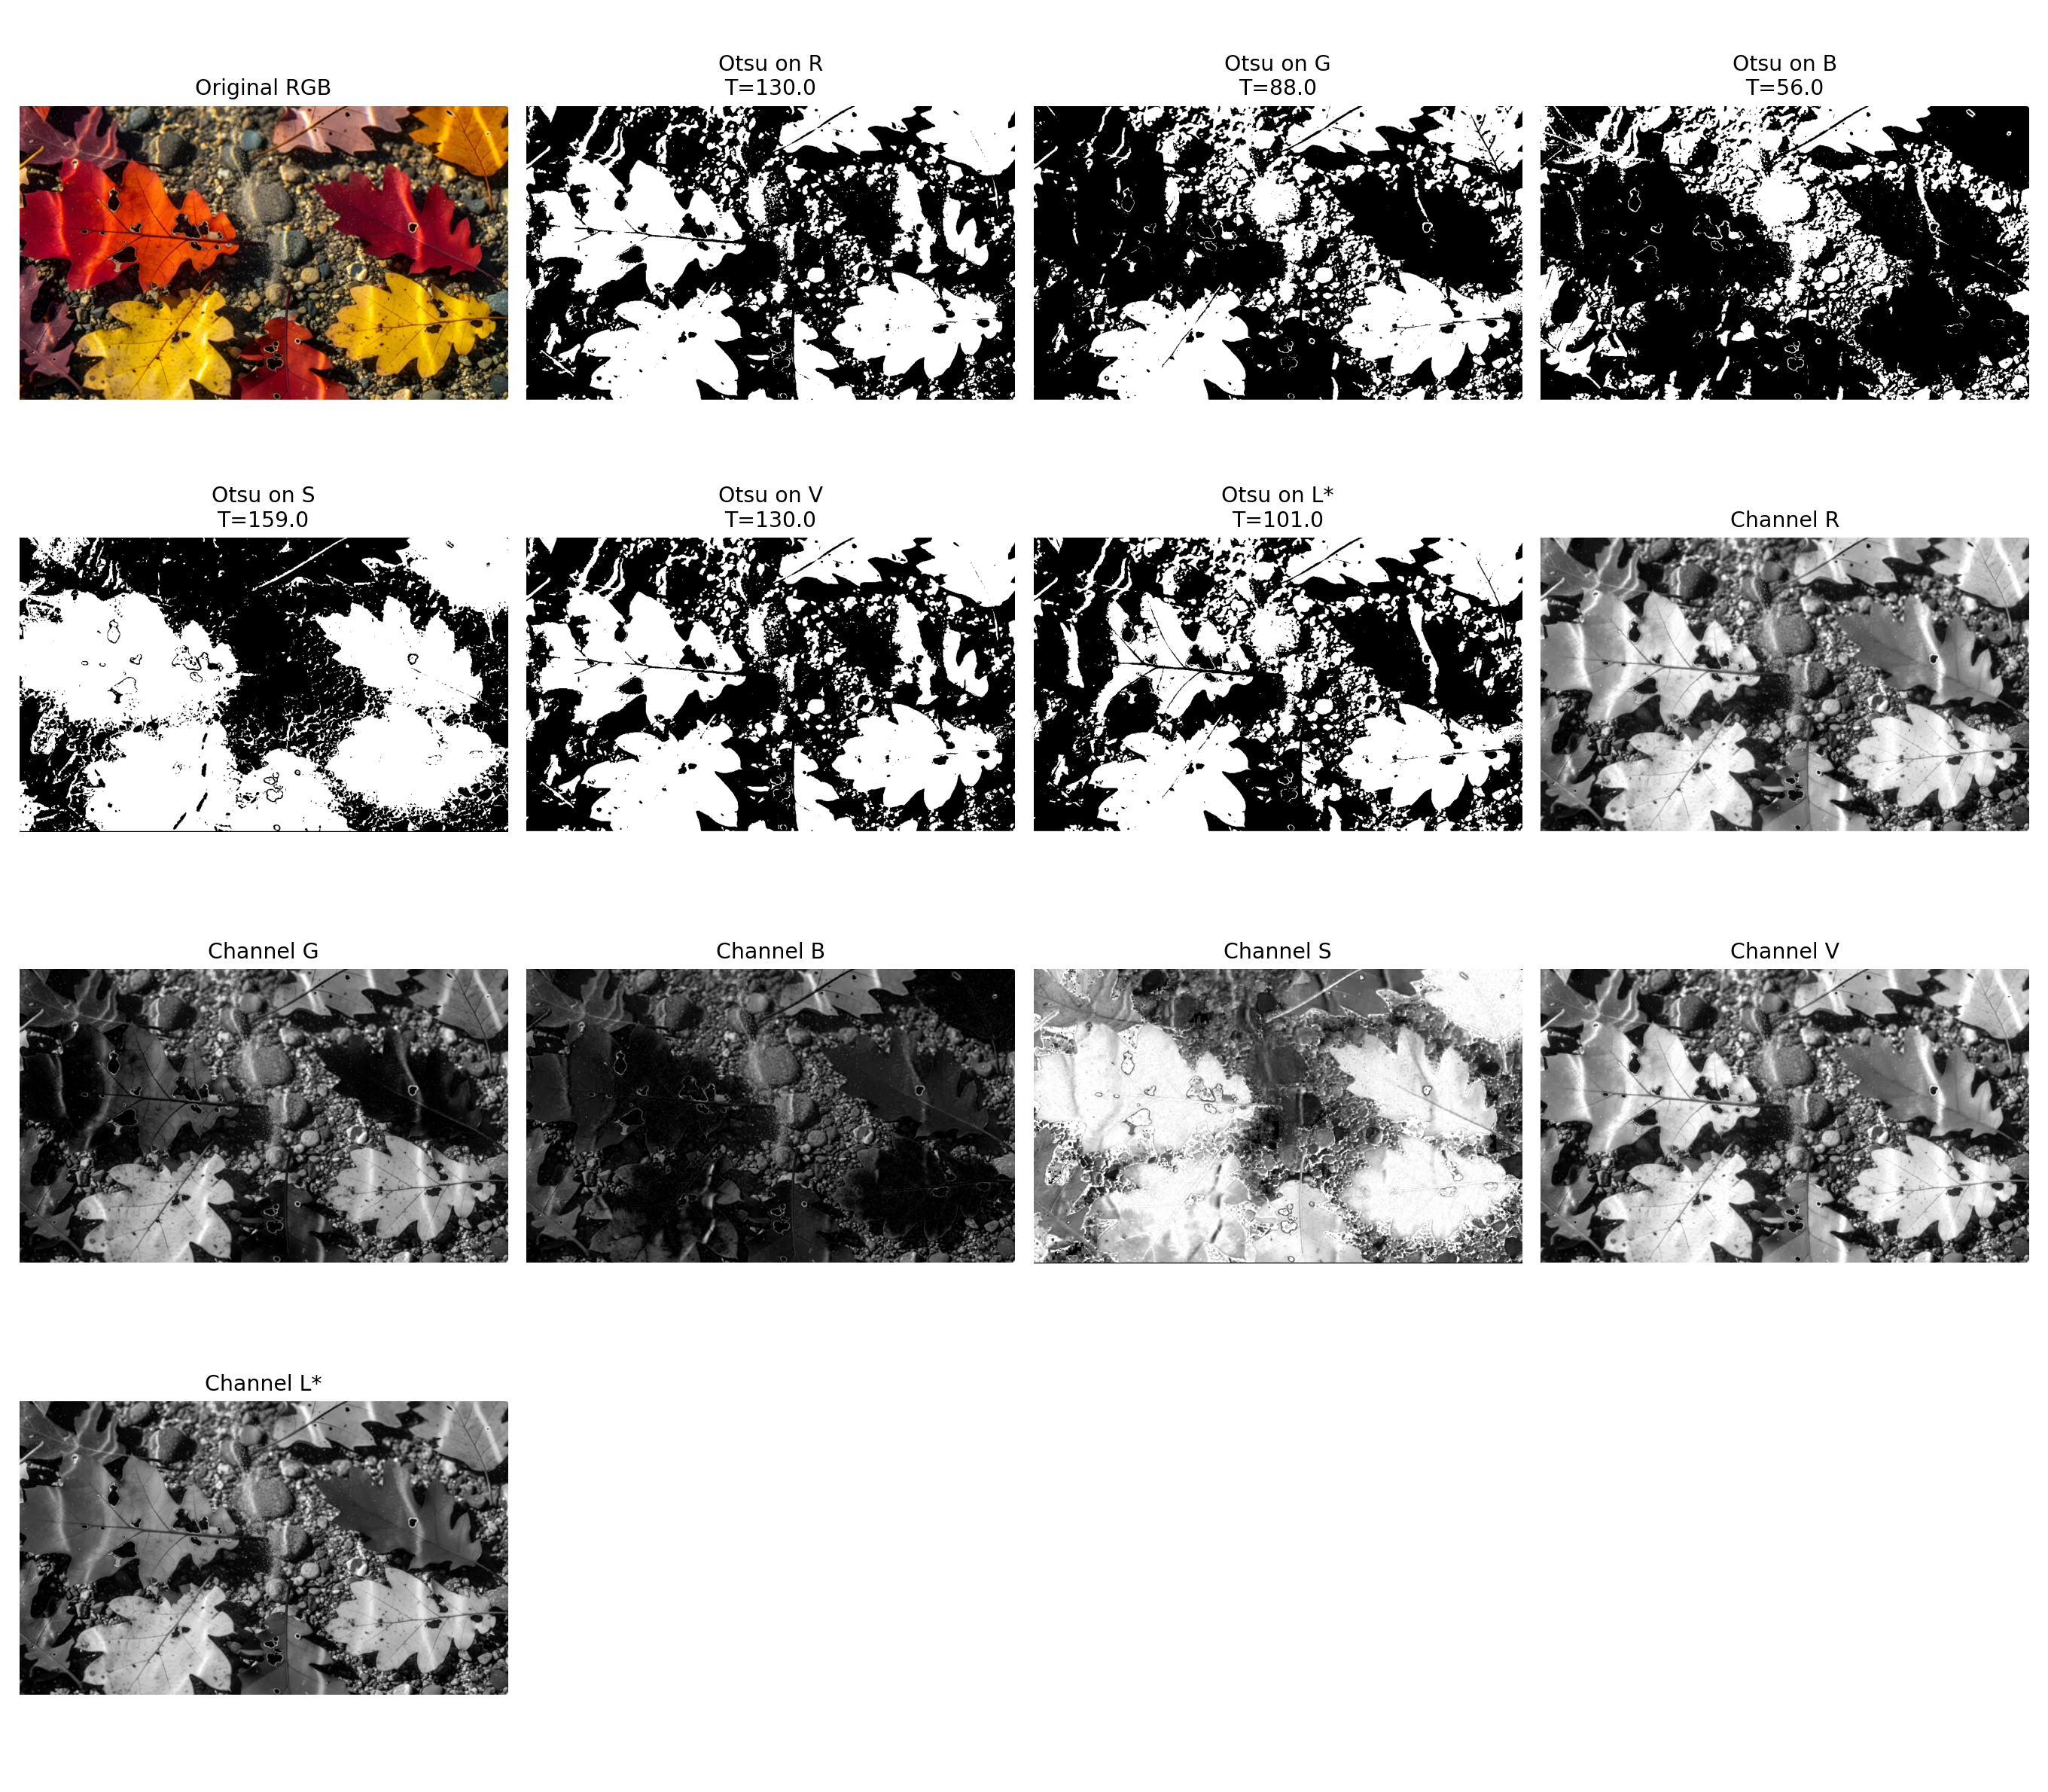
\includegraphics[width=0.97\linewidth]{outputs/otsu_channel_comparison.png}
    \caption{Otsu masks and raw channels for $R,G,B,S,V,L^*$ on \texttt{leaves.png}.}
    \label{fig:otsu_channels}
\end{figure}

\begin{figure}[H]
    \centering
    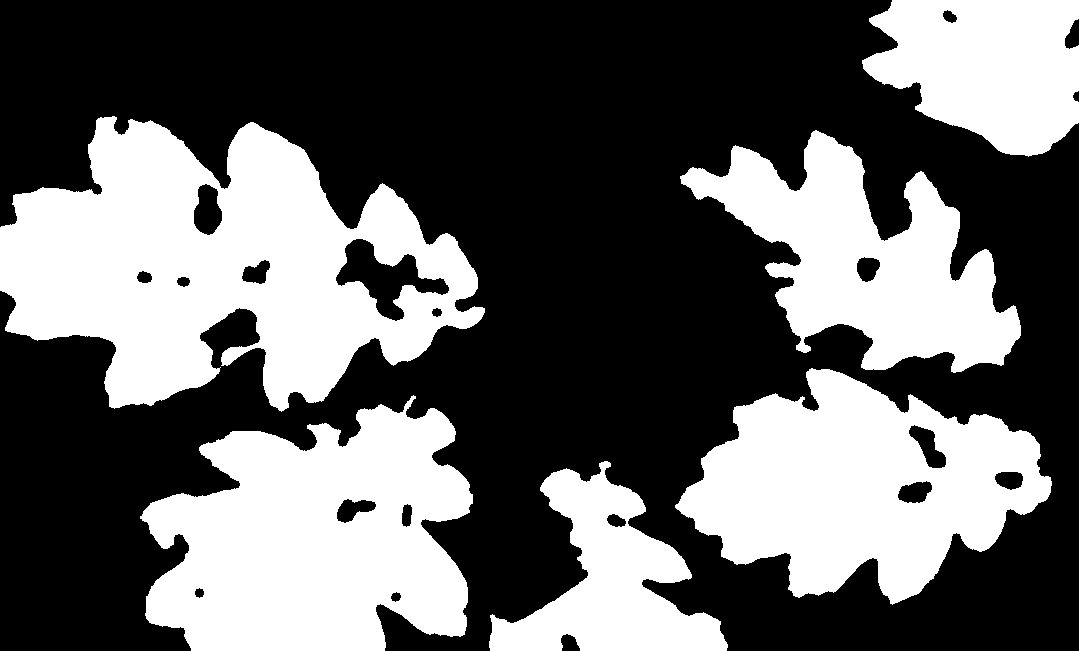
\includegraphics[width=0.75\linewidth]{outputs/mask_pipeline_hsv.png}
    \caption{Two-step HSV auto-thresholding pipeline result.}
    \label{fig:pipeline_hsv}
\end{figure}

\begin{figure}[H]
    \centering
    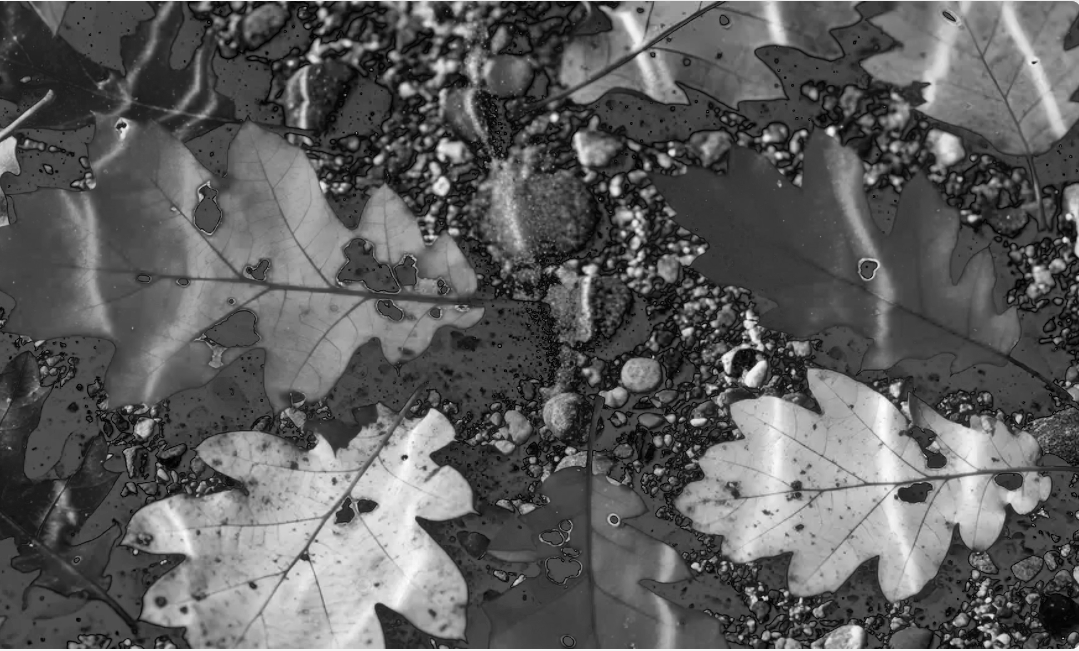
\includegraphics[width=0.75\linewidth]{outputs/distance_image_lab.png}
    \caption{Lab color-distance image and Otsu mask from color-distance thresholding.}
    \label{fig:distance_lab}
\end{figure}

\subsection{Quantitative comparison}

\begin{table}[H]
\centering
\caption{Mask metrics for each thresholding method (values filled from \texttt{outputs/metrics\_summary.csv} after running the notebook).}
\label{tab:metrics}
\begin{tabular}{lccc}
\toprule
\textbf{Method} & \textbf{Threshold} & \textbf{FG ratio} & \textbf{Connected components} \\
\midrule
Otsu-$R$              & (see CSV) & (see CSV) & (see CSV) \\
Otsu-$G$              & (see CSV) & (see CSV) & (see CSV) \\
Otsu-$B$              & (see CSV) & (see CSV) & (see CSV) \\
Otsu-$S$              & (see CSV) & (see CSV) & (see CSV) \\
Otsu-$V$              & (see CSV) & (see CSV) & (see CSV) \\
Otsu-$L^*$            & (see CSV) & (see CSV) & (see CSV) \\
HSV pipeline          & ---       & (see CSV) & (see CSV) \\
Distance + Otsu (Lab) & (see CSV) & (see CSV) & (see CSV) \\
\bottomrule
\end{tabular}
\end{table}

\subsection{Discussion: Otsu on $S$ vs.\ Otsu on $V$}

\subsubsection{When Otsu on $S$ is better}
The saturation channel $S$ attains high values for chromatic (colorful) pixels and low values for achromatic (gray) ones.  When the foreground is colorful and the background is gray or white:
\begin{itemize}
    \item The histogram of $S$ is \emph{bimodal}: one peak near 0 (gray background) and one peak at higher saturation (colored object).
    \item Otsu finds a clear valley between the two classes, producing a clean mask.
    \item Illumination changes that scale $V$ uniformly do not affect $S$, making it more robust.
\end{itemize}

\subsubsection{When Otsu on $V$ (or $L^*$) is better}
The value / luminance channel captures brightness.  When:
\begin{itemize}
    \item Both foreground and background are near gray (low saturation), the $S$ channel collapses to near zero and offers no class separation.
    \item The key discriminant is a strong brightness contrast (e.g.\ bright tablets on a dark background).
    \item $V$ (or $L^*$) then provides the only bi-modal histogram suitable for Otsu.
\end{itemize}
In practice, combining both steps (Otsu on $S$ then on $V$) as in the HSV pipeline gives the most robust result.

% ============================================================
\section{Task 6.5 — Color Edge Detection}
% ============================================================

\subsection{Theoretical background}

\subsubsection{Multi-channel Canny}
Run the standard Canny detector independently on each scalar channel ($R$, $G$, $B$) and merge the binary edge maps with a pixel-wise OR:
\[
E_{\mathrm{multi}}(x,y) = E_R \vee E_G \vee E_B.
\]
\textbf{Advantage:} simple.  \textbf{Disadvantage:} may produce redundant edges; edge direction is undefined.

\subsubsection{Di Zenzo color gradient magnitude}
Model the image as a vector field $\mathbf{I}=(I_1,I_2,I_3)^\top$.  Define partial derivatives $\mathbf{I}_x$ and $\mathbf{I}_y$ (one per channel).  Build the $2\times2$ structure tensor
\[
\mathbf{G} = \begin{bmatrix} g_{xx} & g_{xy} \\ g_{xy} & g_{yy} \end{bmatrix},
\quad
g_{xx}=\mathbf{I}_x^\top\mathbf{I}_x,\;
g_{yy}=\mathbf{I}_y^\top\mathbf{I}_y,\;
g_{xy}=\mathbf{I}_x^\top\mathbf{I}_y.
\]
The maximum-directional derivative magnitude is
\[
M(x,y)=\sqrt{\frac{g_{xx}+g_{yy}+\sqrt{(g_{xx}-g_{yy})^2+4g_{xy}^2}}{2}},
\]
and the corresponding edge direction is
\[
\theta = \tfrac{1}{2}\arctan\!\left(\frac{2g_{xy}}{g_{xx}-g_{yy}+\varepsilon}\right).
\]

\subsubsection{Non-maximum suppression (NMS) and hysteresis}
The same NMS and double-threshold hysteresis steps from classical Canny are applied to $M$ and $\theta$ to produce a thinned, connected edge map --- completing a ``mini color Canny.''

\subsection{Results}

\begin{figure}[H]
    \centering
    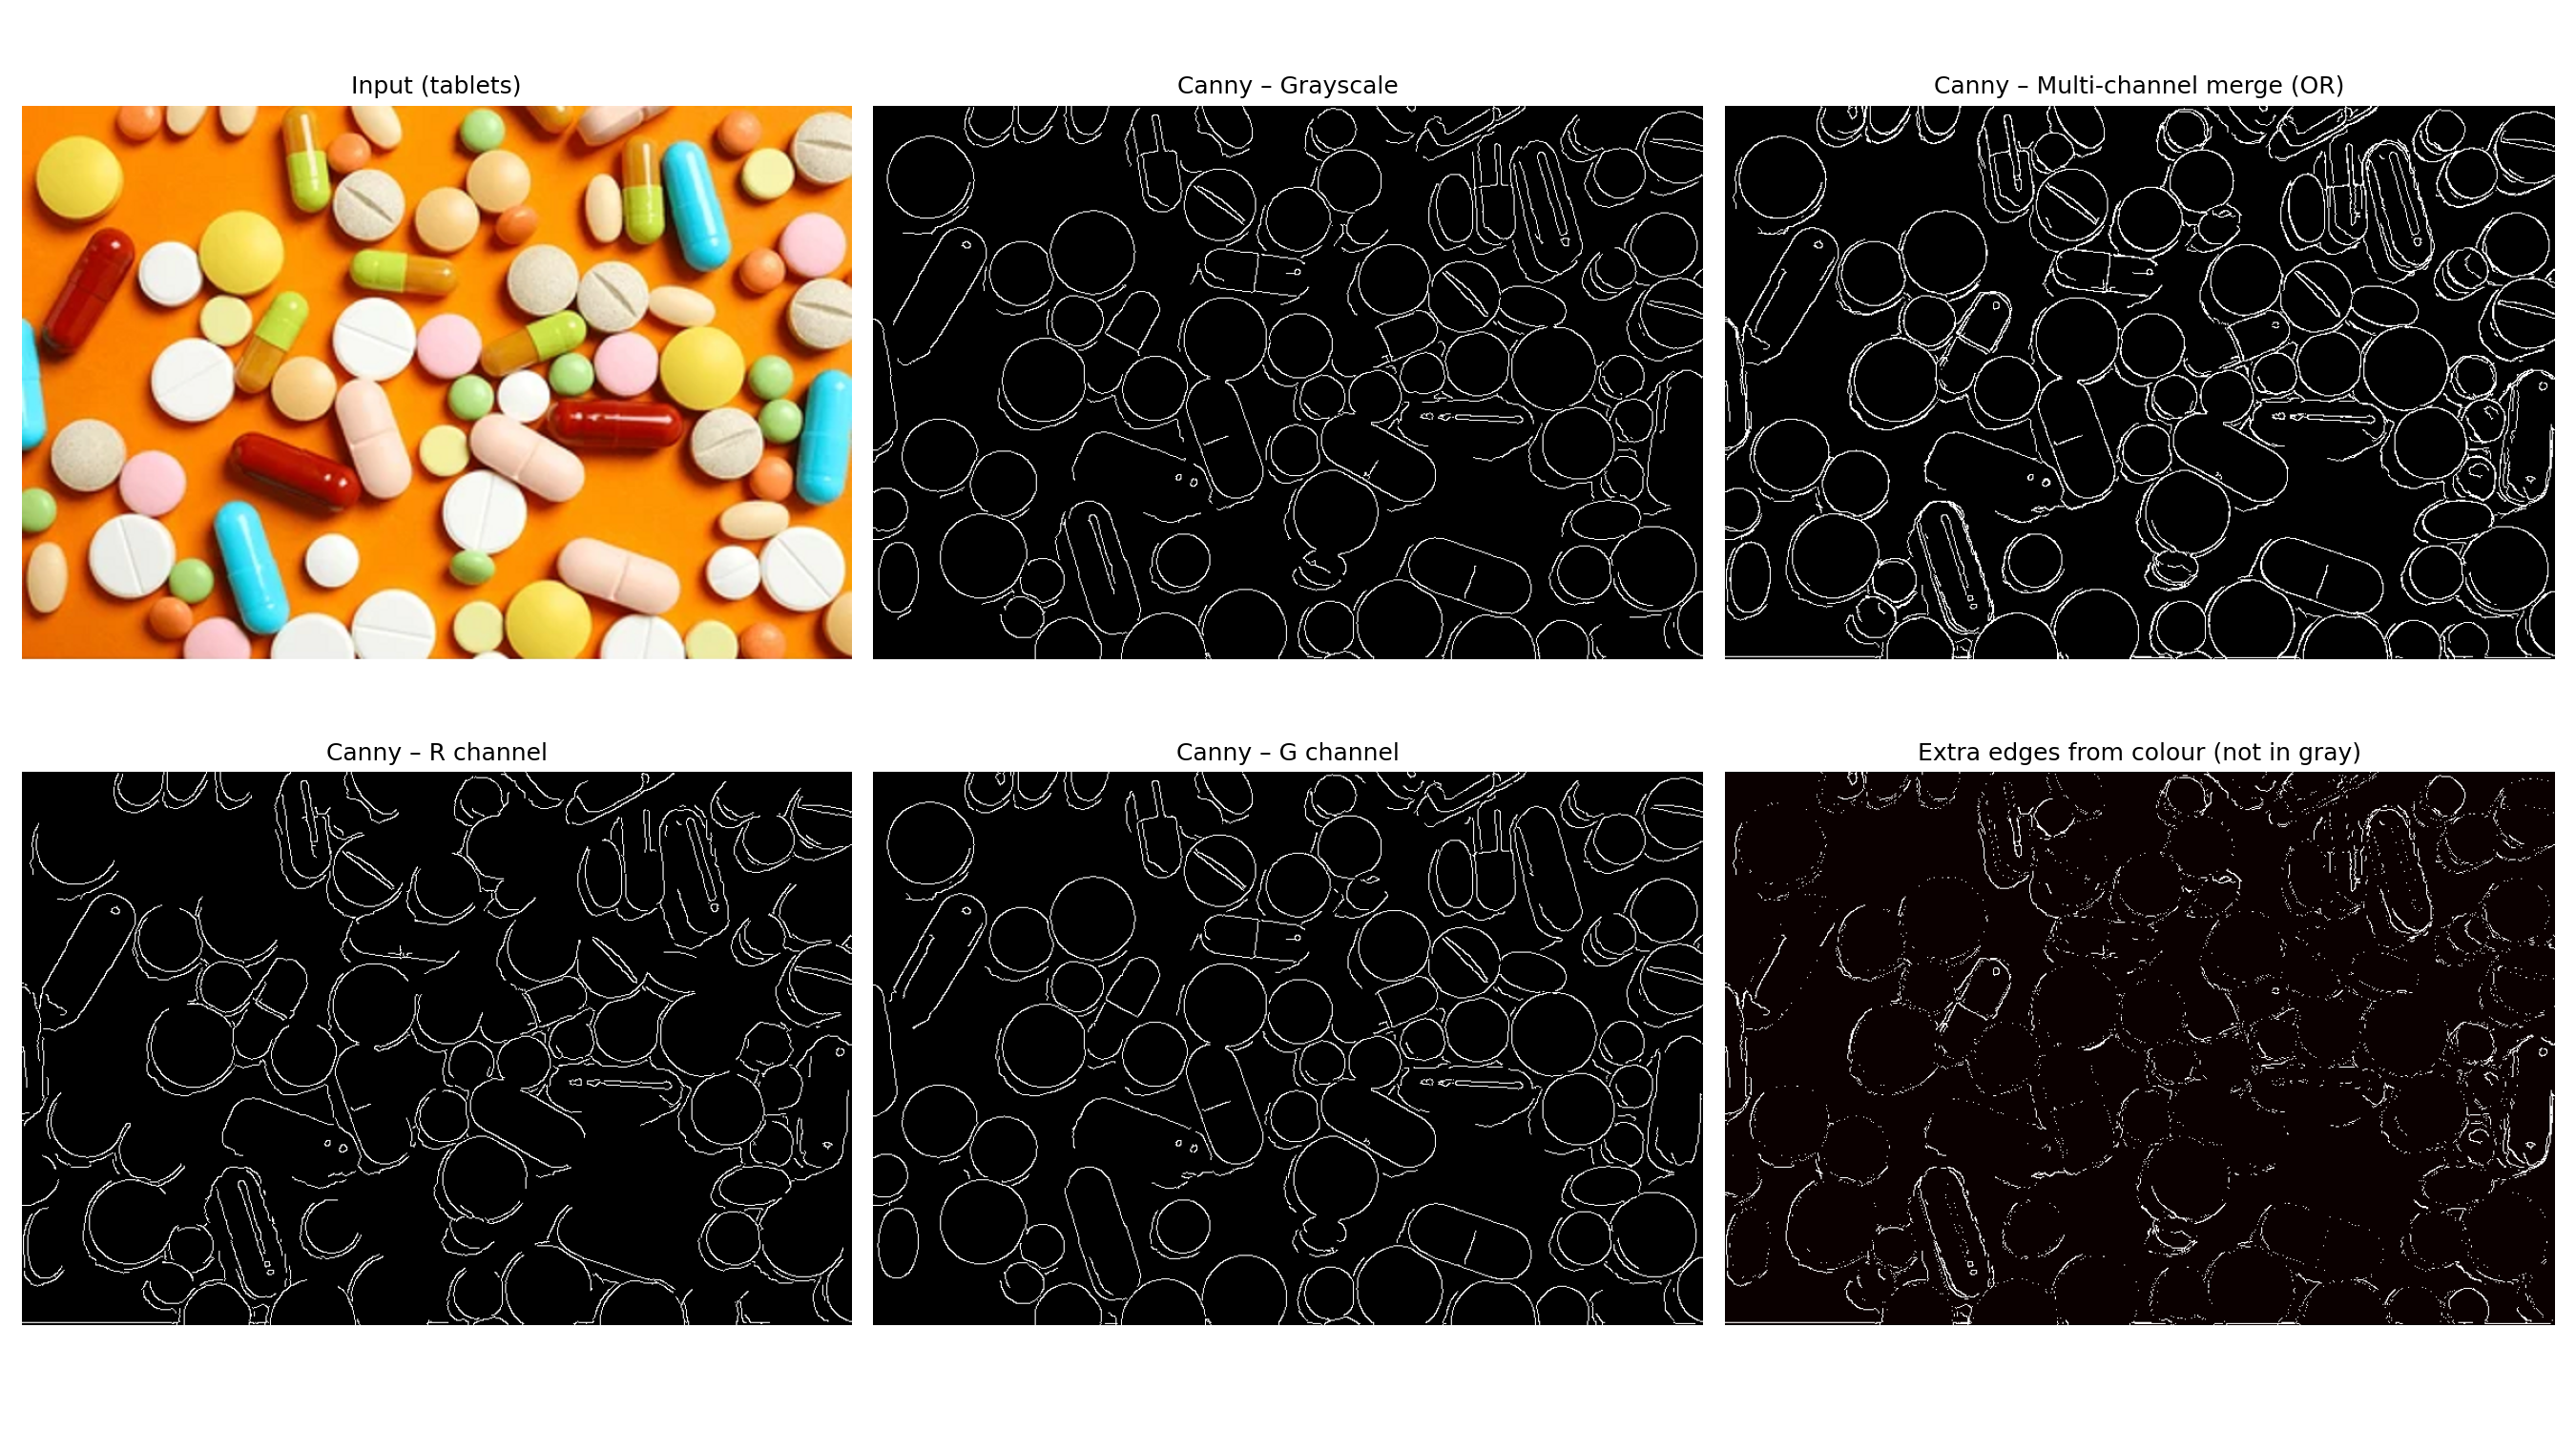
\includegraphics[width=0.97\linewidth]{outputs/canny_multichannel_vs_gray.png}
    \caption{Multi-channel Canny vs.\ grayscale Canny on \texttt{tablets4.png}. The heat map in the last panel shows edges detected by color but not by grayscale.}
    \label{fig:multichannel_canny}
\end{figure}

\begin{figure}[H]
    \centering
    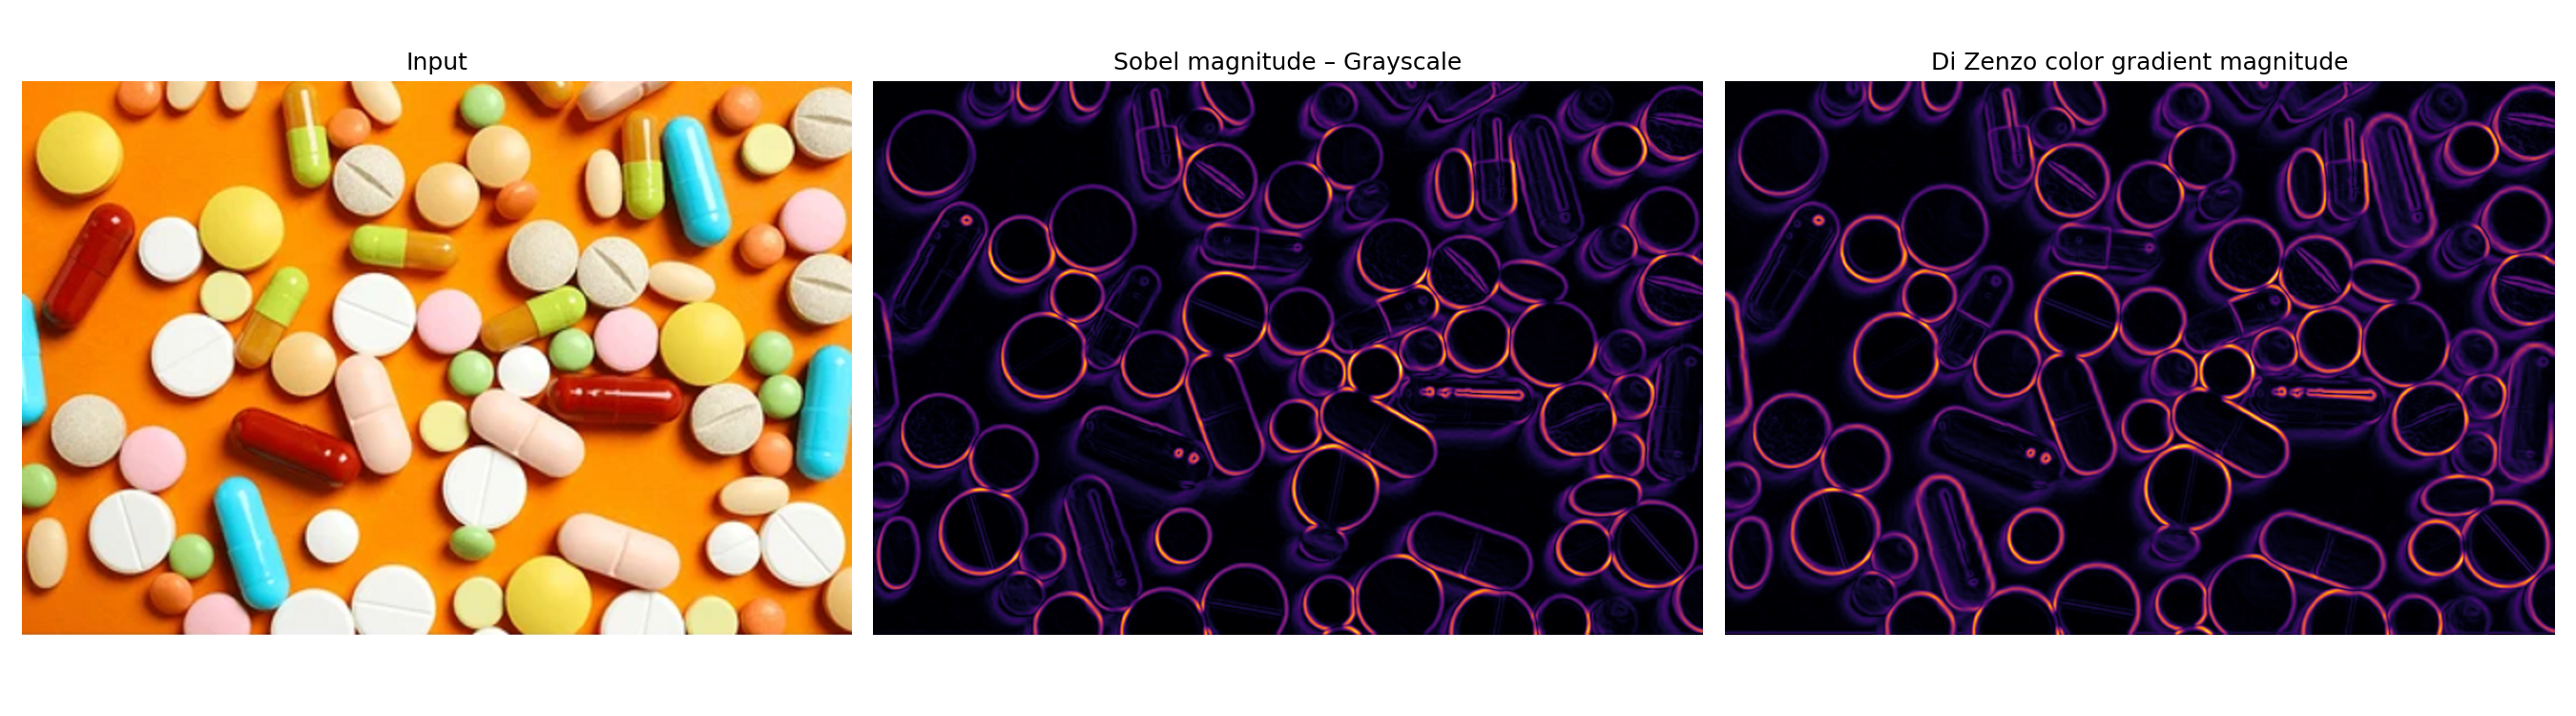
\includegraphics[width=0.75\linewidth]{outputs/color_gradient_magnitude.png}
    \caption{Di~Zenzo color gradient magnitude vs.\ Sobel gradient on grayscale.}
    \label{fig:color_gradient}
\end{figure}

\begin{figure}[H]
    \centering
    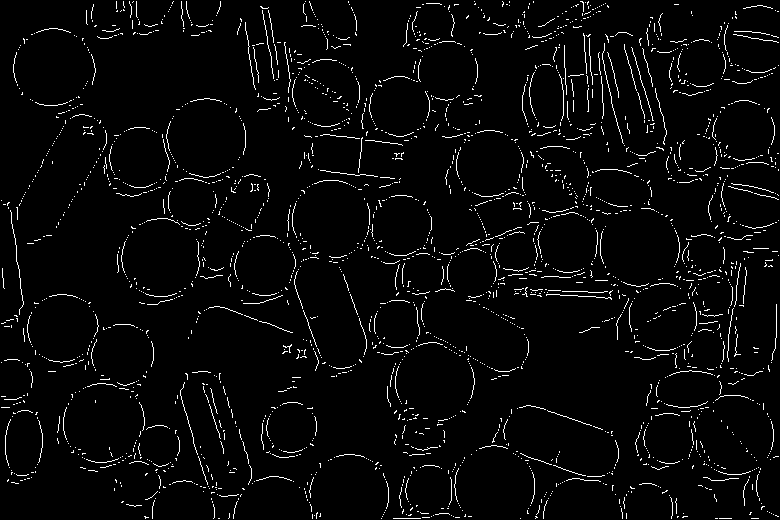
\includegraphics[width=0.75\linewidth]{outputs/mini_color_canny.png}
    \caption{Mini color Canny (NMS + hysteresis) vs.\ standard grayscale Canny.}
    \label{fig:mini_canny}
\end{figure}

\begin{figure}[H]
    \centering
    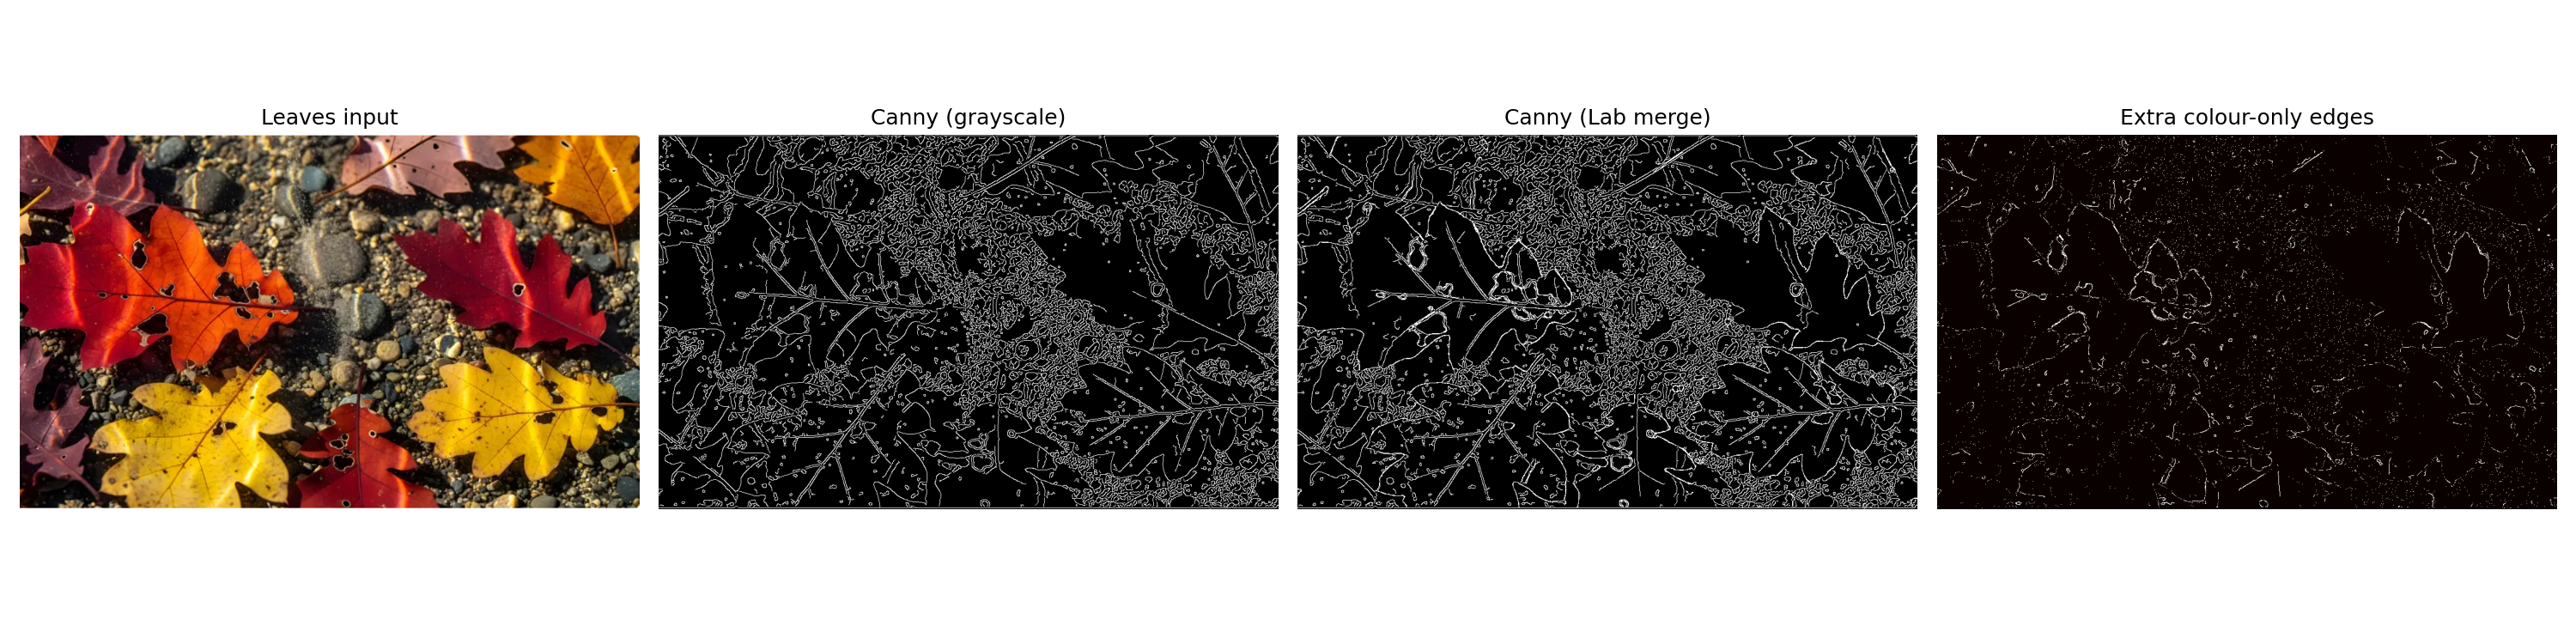
\includegraphics[width=0.97\linewidth]{outputs/colour_edges_vs_gray_leaves.png}
    \caption{Leaves image: edges found by color-Lab Canny but missed by grayscale Canny (heat map on the right).}
    \label{fig:color_vs_gray_leaves}
\end{figure}

\subsection{Analysis}

The Di~Zenzo magnitude detects boundaries arising from \emph{any} color channel, including those invisible in grayscale.  On the leaves image, boundaries between same-brightness but differently-hued leaves are absent in the grayscale Canny result but clearly present in the color variant (Figure~\ref{fig:color_vs_gray_leaves}).  The mini color Canny adds NMS to thin the edges, reducing false activations from the raw magnitude thresholding.

% ============================================================
\section{Task 7.5 — Region-Based Color Segmentation}
% ============================================================

\subsection{Theoretical background}

\subsubsection{Region growing}
Starting from a seed pixel $s$, a region $R$ is grown by repeatedly adding unvisited neighbors satisfying:
\[
\bigl\|\mathbf{c}(x,y) - \boldsymbol{\mu}_R\bigr\|_2 \le T,
\]
where $\boldsymbol{\mu}_R$ is the running mean color of the region.

Lab space is preferred because Euclidean distance in Lab approximates perceptual color difference (CIE76), while Euclidean distance in RGB does not account for human vision non-linearity.

\subsubsection{K-means color clustering}
Pixel feature vector:
\[
\mathbf{f}(x,y) = \bigl[L^*/100,\; a^*/128,\; b^*/128,\; \lambda x/W,\; \lambda y/H\bigr]^\top,
\]
where $\lambda$ is a spatial weight ($0.5$ used here).  Adding $(x,y)$ strongly encourages spatially contiguous segments.

\subsubsection{Split-and-merge variance criterion}
A region $R$ is considered \emph{homogeneous} if
\[
\max_c \mathrm{Var}_c(R) < T_{\sigma^2},
\]
where $c$ indexes Lab channels.  If the criterion fails, $R$ is split into four quadrants.  Adjacent homogeneous regions with similar mean color are merged.

\subsection{Results}

\begin{figure}[H]
    \centering
    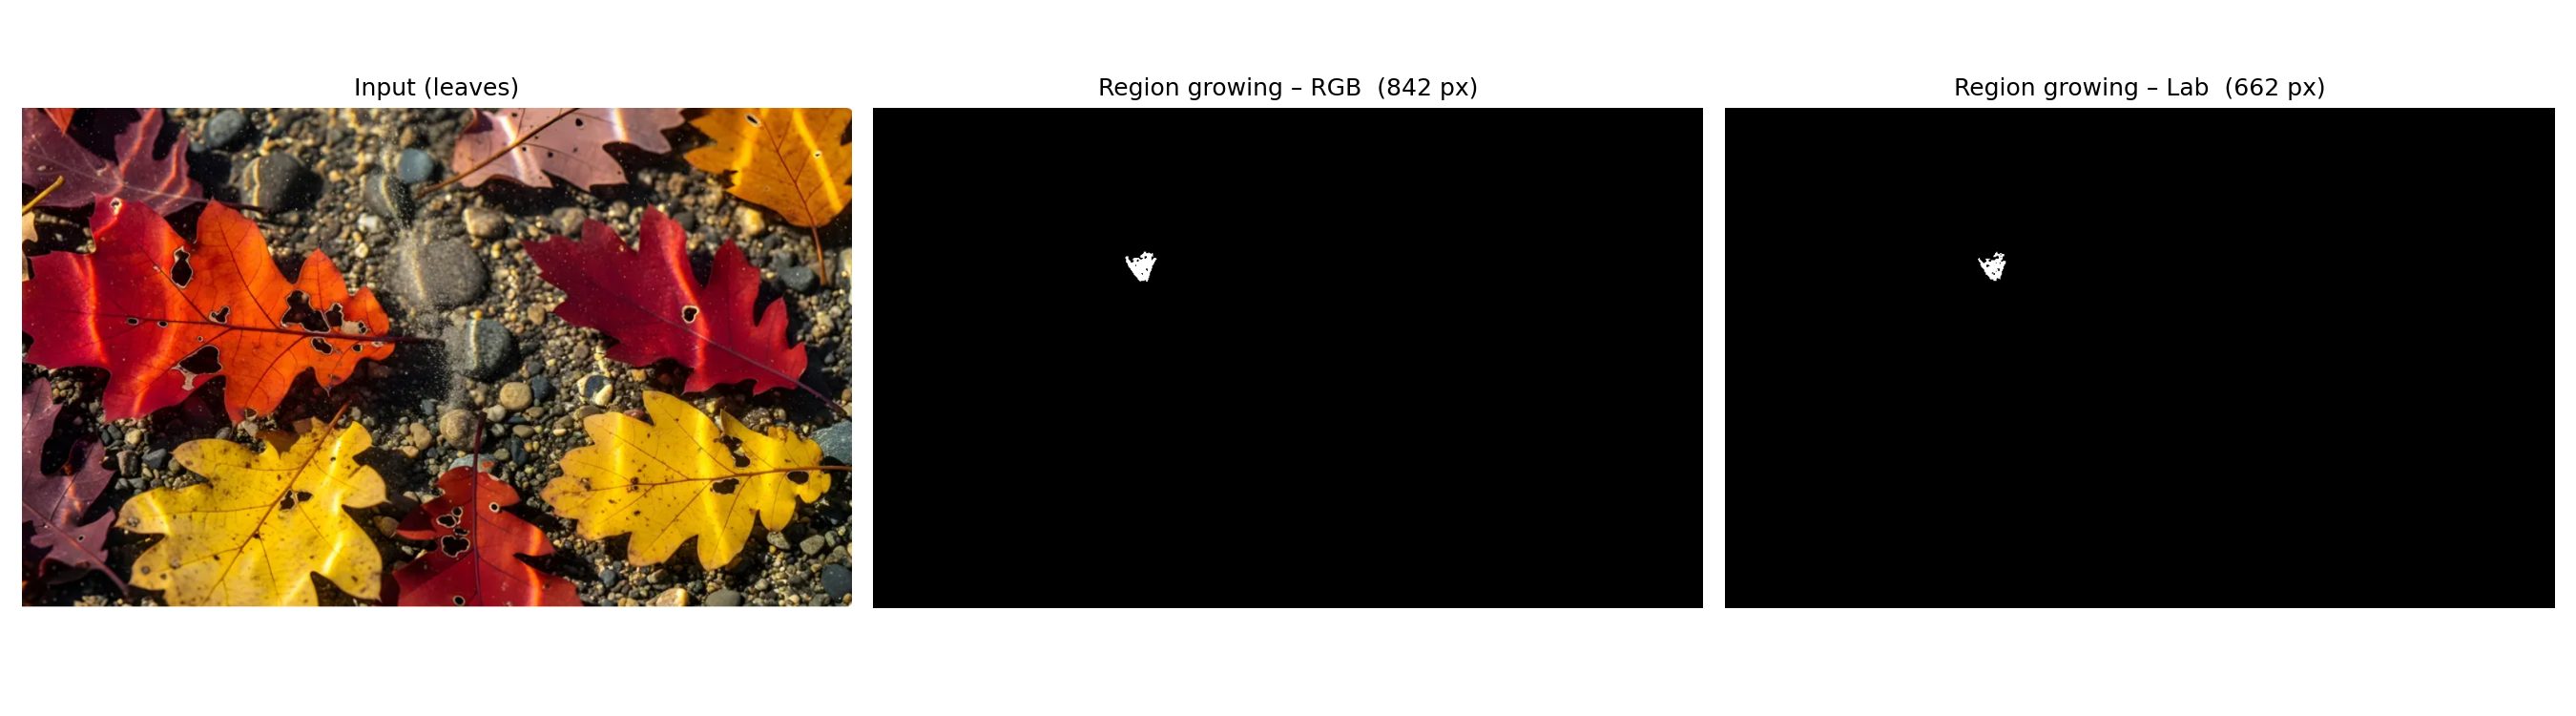
\includegraphics[width=0.97\linewidth]{outputs/region_growing_rgb_vs_lab.png}
    \caption{Region growing from a single seed in RGB (scaled) vs.\ Lab on \texttt{leaves.png}.}
    \label{fig:rg_rgb_lab}
\end{figure}

\begin{figure}[H]
    \centering
    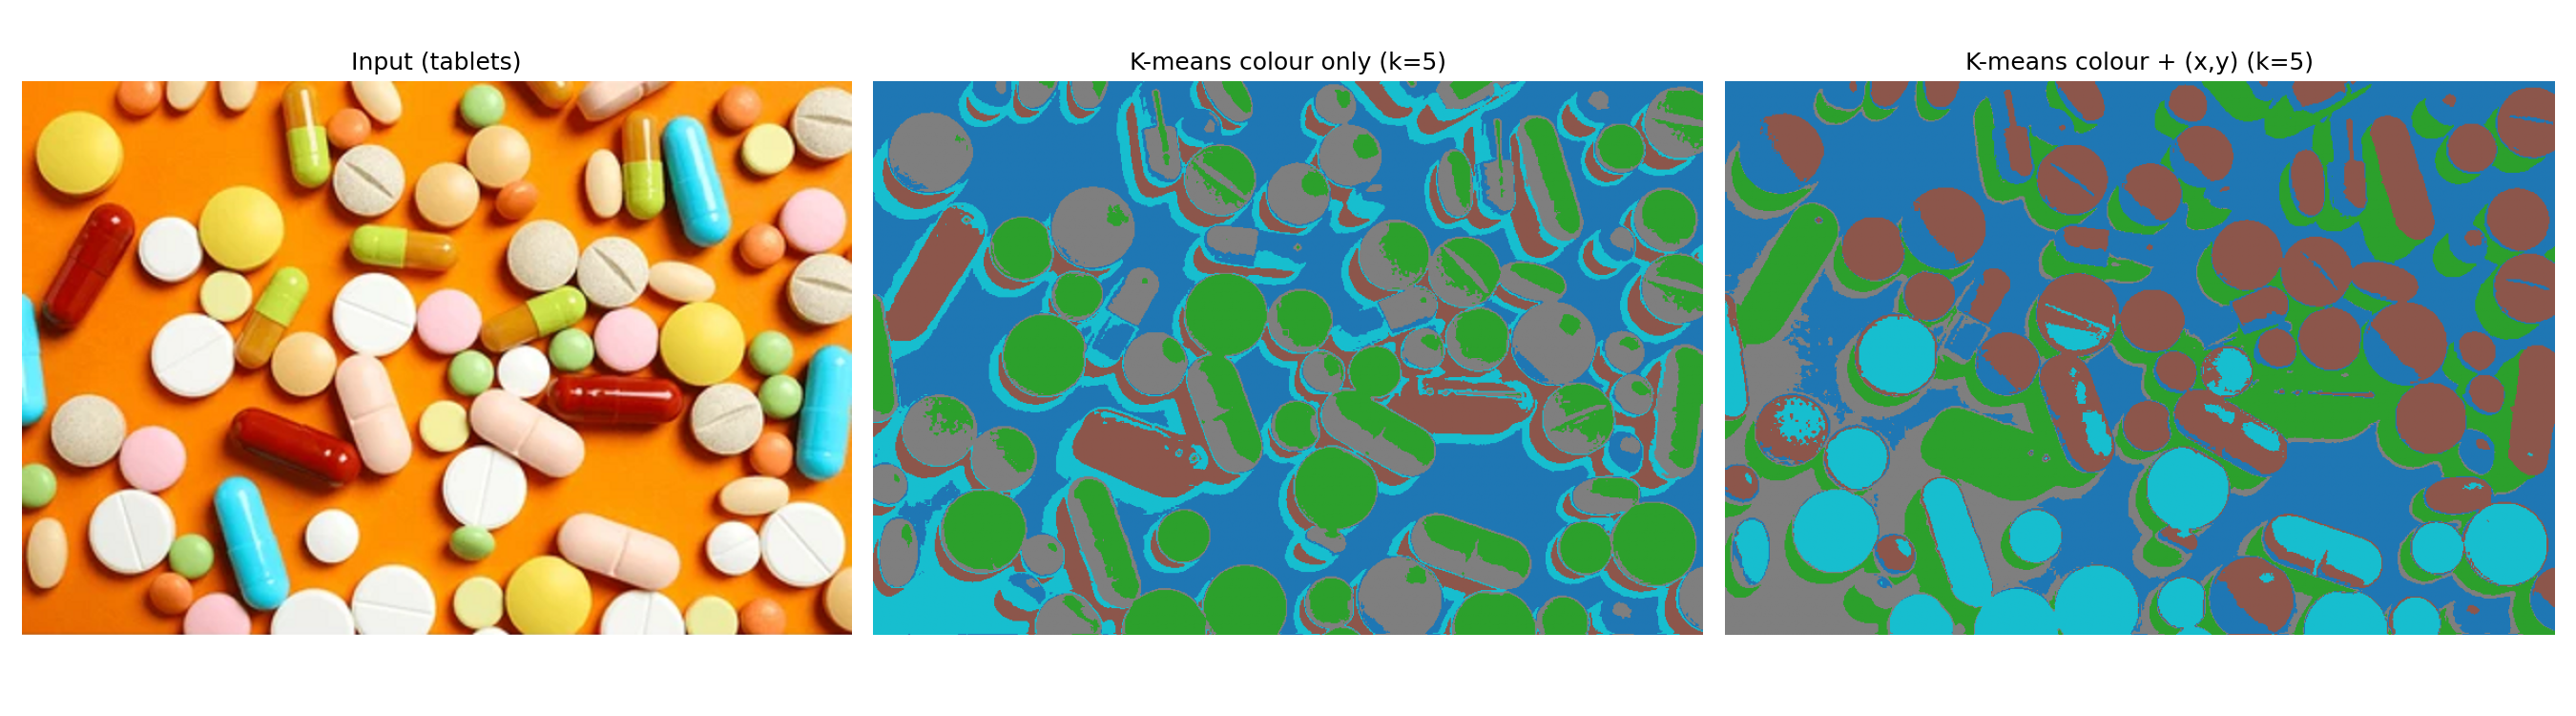
\includegraphics[width=0.75\linewidth]{outputs/kmeans_colour_vs_xy.png}
    \caption{K-means segmentation: color only (left) vs.\ color + position (right) on \texttt{tablets4.png}.}
    \label{fig:kmeans}
\end{figure}

\begin{figure}[H]
    \centering
    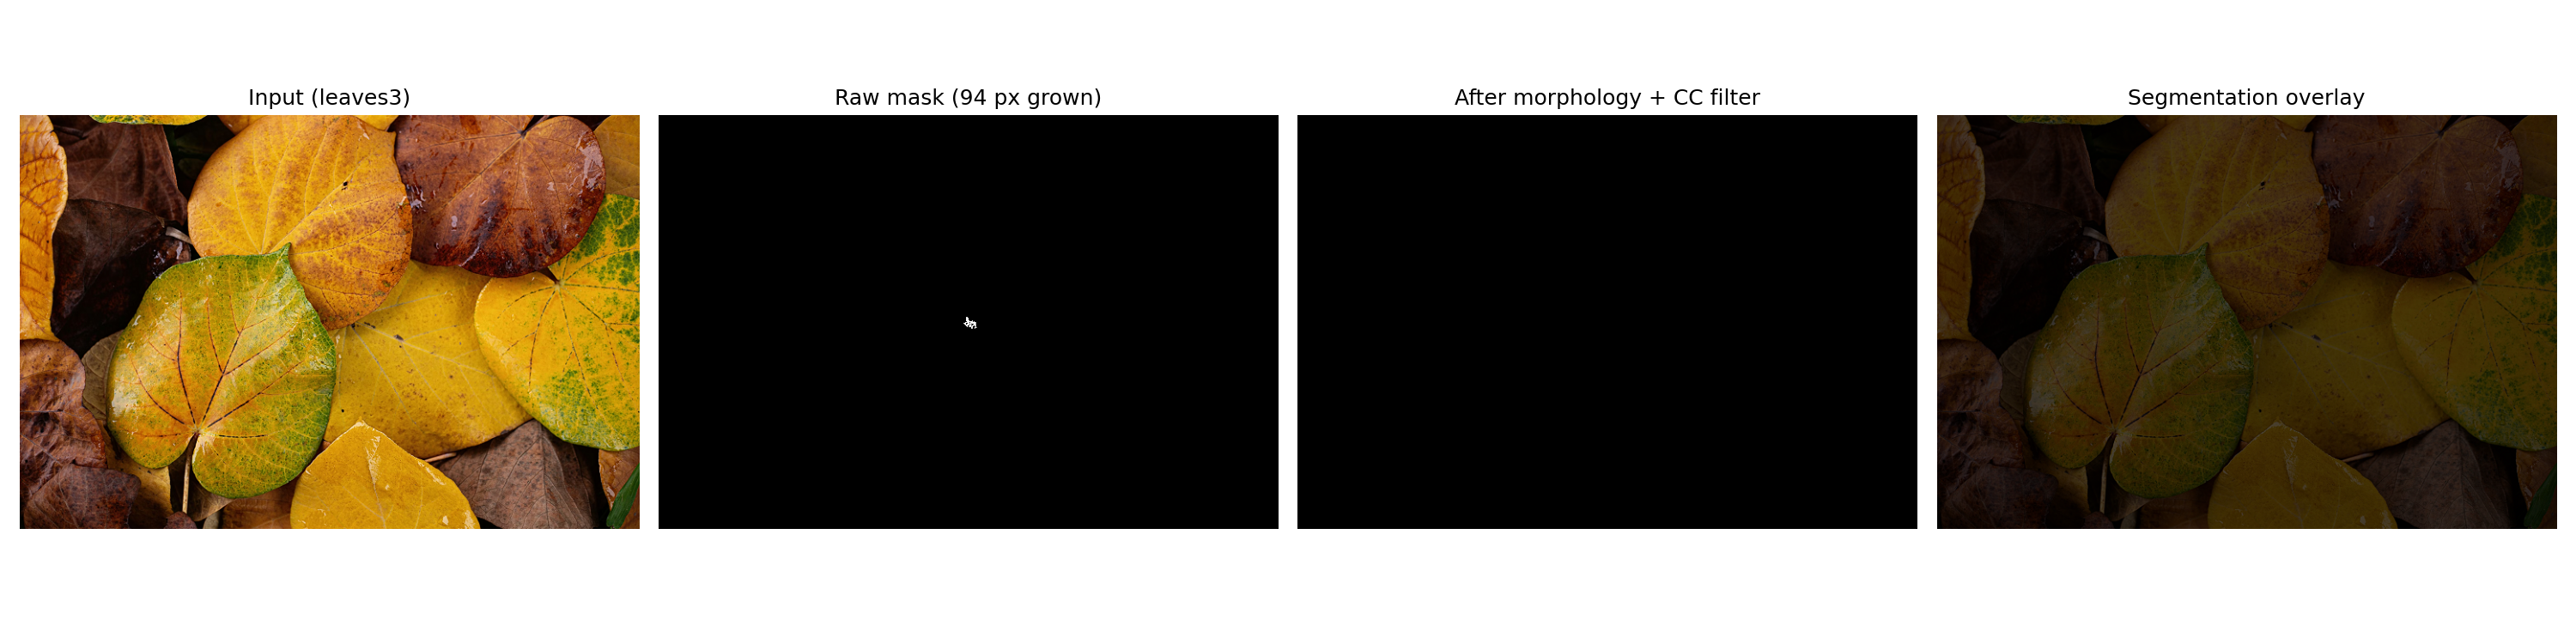
\includegraphics[width=0.97\linewidth]{outputs/leaf_region_growing_pipeline.png}
    \caption{Leaf segmentation pipeline: region growing in Lab + morphology + connected-component filter.}
    \label{fig:leaf_pipeline}
\end{figure}

\begin{figure}[H]
    \centering
    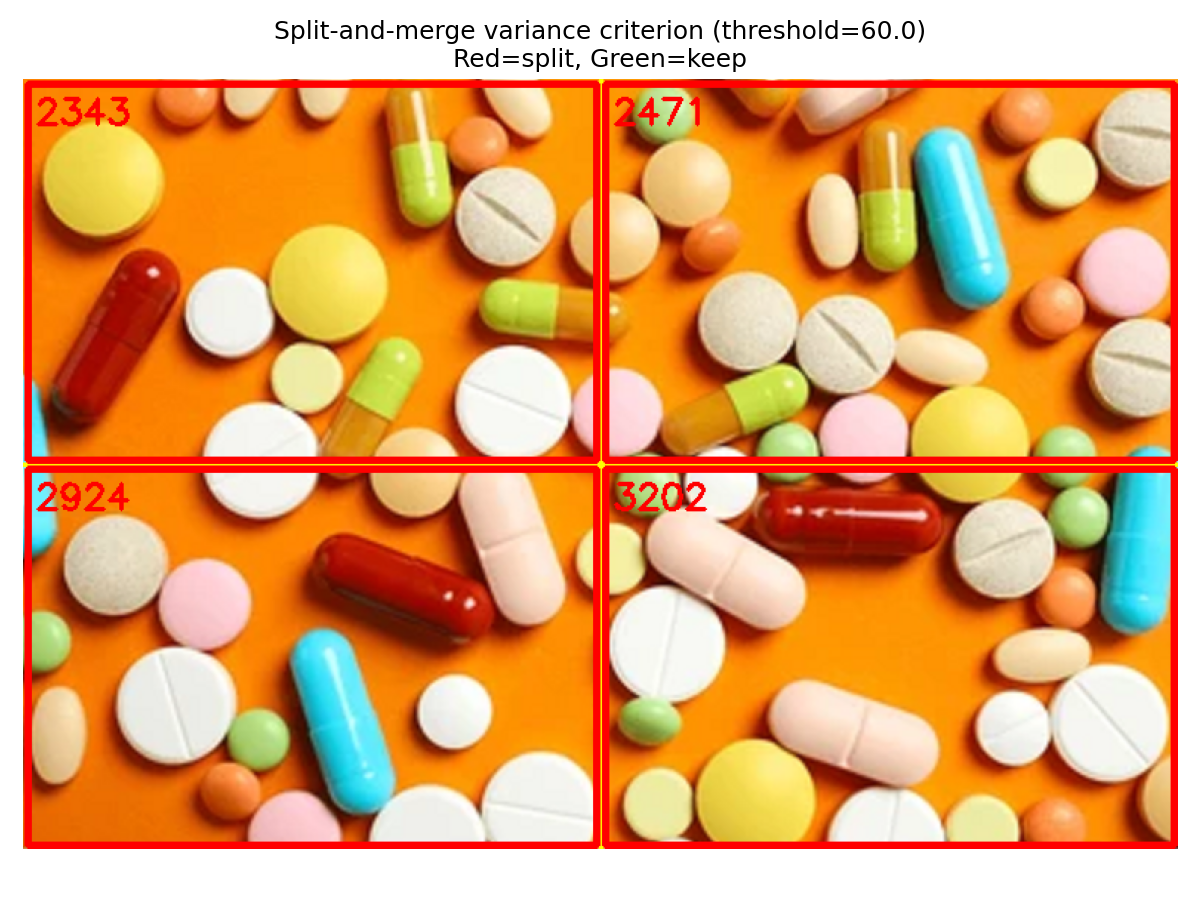
\includegraphics[width=0.55\linewidth]{outputs/split_merge_variance.png}
    \caption{Split-and-merge variance criterion visualized on quadrants of \texttt{tablets4.png}. Red border = variance above threshold (needs splitting); green = homogeneous leaf.}
    \label{fig:split_merge}
\end{figure}

\subsection{Discussion}

\textbf{RGB vs.\ Lab in region growing.}
In RGB, all three channels are correlated with luminance, so similar-brightness pixels of different hues may be incorrectly merged.  Lab separates luminance ($L^*$) from chrominance ($a^*$, $b^*$), so the threshold $T$ applies more uniformly across color directions.  Region growing in Lab therefore produces more stable results for a fixed $T$ when illumination is uneven.

\textbf{K-means with and without position.}
Without spatial features, K-means groups disconnected pixels of the same color into the same cluster.  Adding $(x,y)$ introduces a ``gravity'' towards spatially nearby pixels, producing compact regions.  The trade-off is that large objects of the same color may be split if they are spatially spread.

% ============================================================
\section{Task 8.5 — Edge-Based Color Segmentation}
% ============================================================

\subsection{Theoretical background}

\subsubsection{Canny on individual color-space channels}
Running Canny on $L^*$ detects luminance boundaries; running it on $S$ detects saturation transitions (e.g.\ edges of colorful objects against muted backgrounds).  Merging these maps with OR captures a wider set of meaningful boundaries.

\subsubsection{Edge-to-region pipeline}
\begin{enumerate}
    \item Detect color edges (Canny on $L^* \vee S$, or Di~Zenzo threshold).
    \item Morphological \textsc{close} to seal small gaps in contours.
    \item \texttt{findContours} with \texttt{RETR\_EXTERNAL} and fill interiors (\texttt{FILLED}).
    \item Area filter to remove small spurious regions.
\end{enumerate}

\subsubsection{Active contour with color edge map}
The standard snake energy is augmented with a color edge force:
\[
E_{\mathrm{image}} = w_1|\nabla L^*| + w_2|\nabla S| + w_3 M_{\mathrm{DiZenzo}}.
\]
For a geodesic active contour / level set, the stopping function is
\[
g(x,y) = \frac{1}{1 + \alpha\, M(x,y)^2}, \quad \alpha > 0,
\]
which is close to 0 on strong color edges and close to 1 in flat regions, naturally stopping the curve at color boundaries.

\subsection{Results}

\begin{figure}[H]
    \centering
    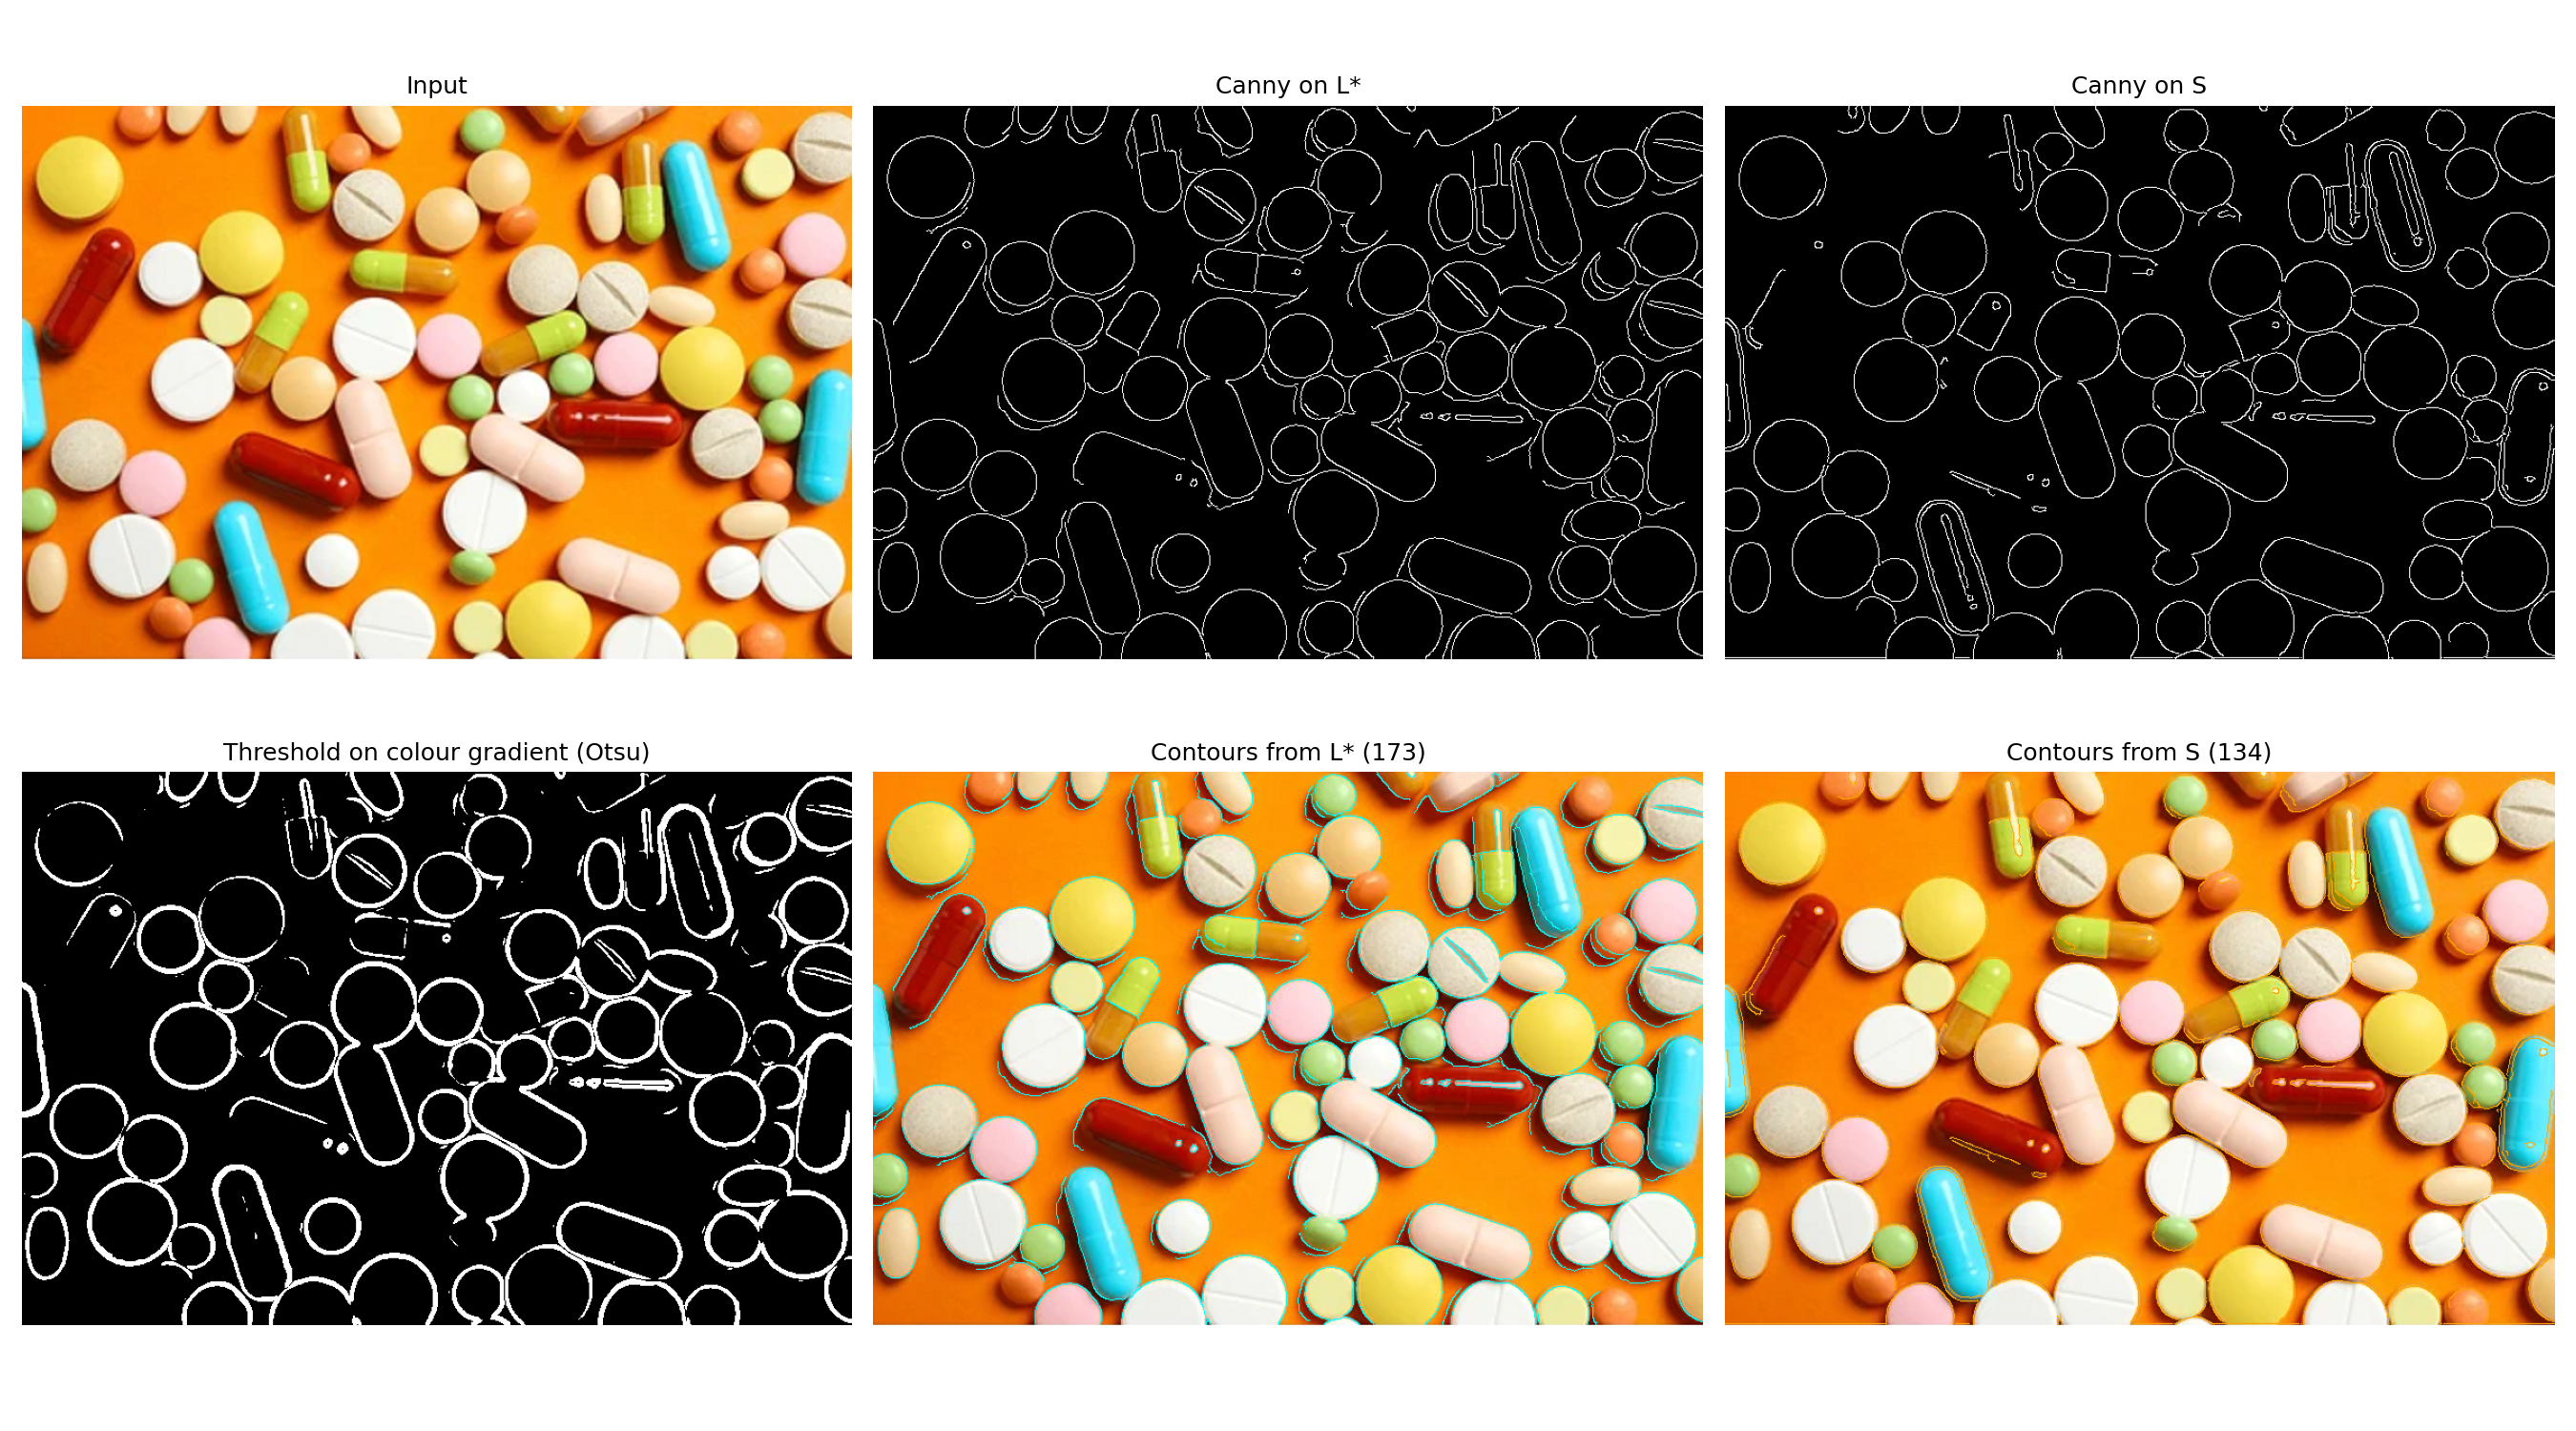
\includegraphics[width=0.97\linewidth]{outputs/edge_canny_L_S_colourgrad.png}
    \caption{Edge maps from Canny on $L^*$ and $S$, and contours drawn on the input image (\texttt{tablets4.png}).}
    \label{fig:edge_L_S}
\end{figure}

\begin{figure}[H]
    \centering
    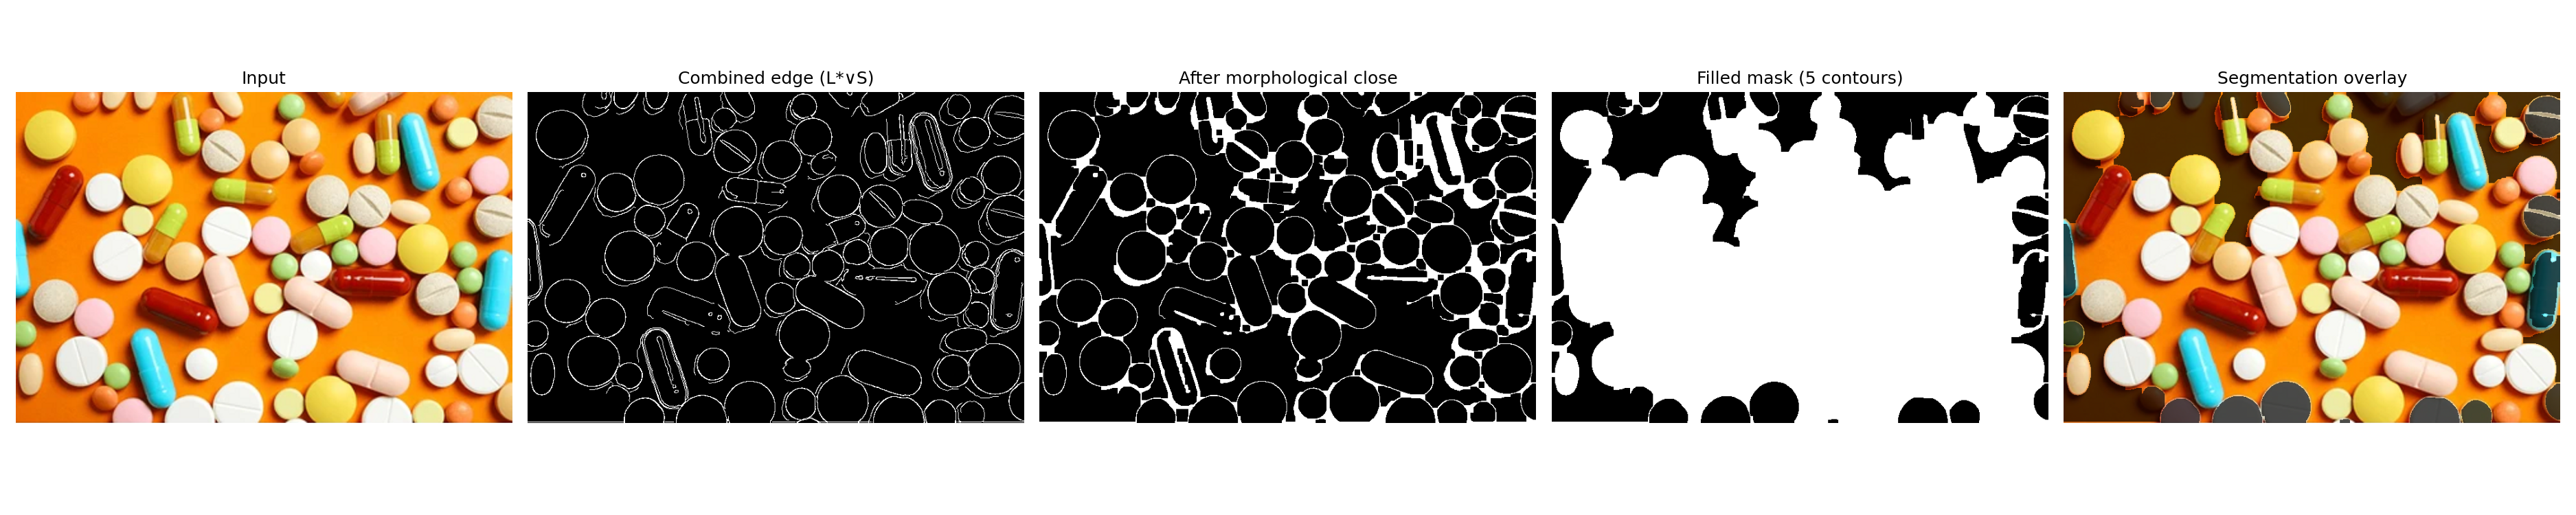
\includegraphics[width=0.97\linewidth]{outputs/edge_to_region_pipeline.png}
    \caption{Color edge $\to$ morphological close $\to$ filled contour mask $\to$ segmentation overlay.}
    \label{fig:edge_region}
\end{figure}

\begin{figure}[H]
    \centering
    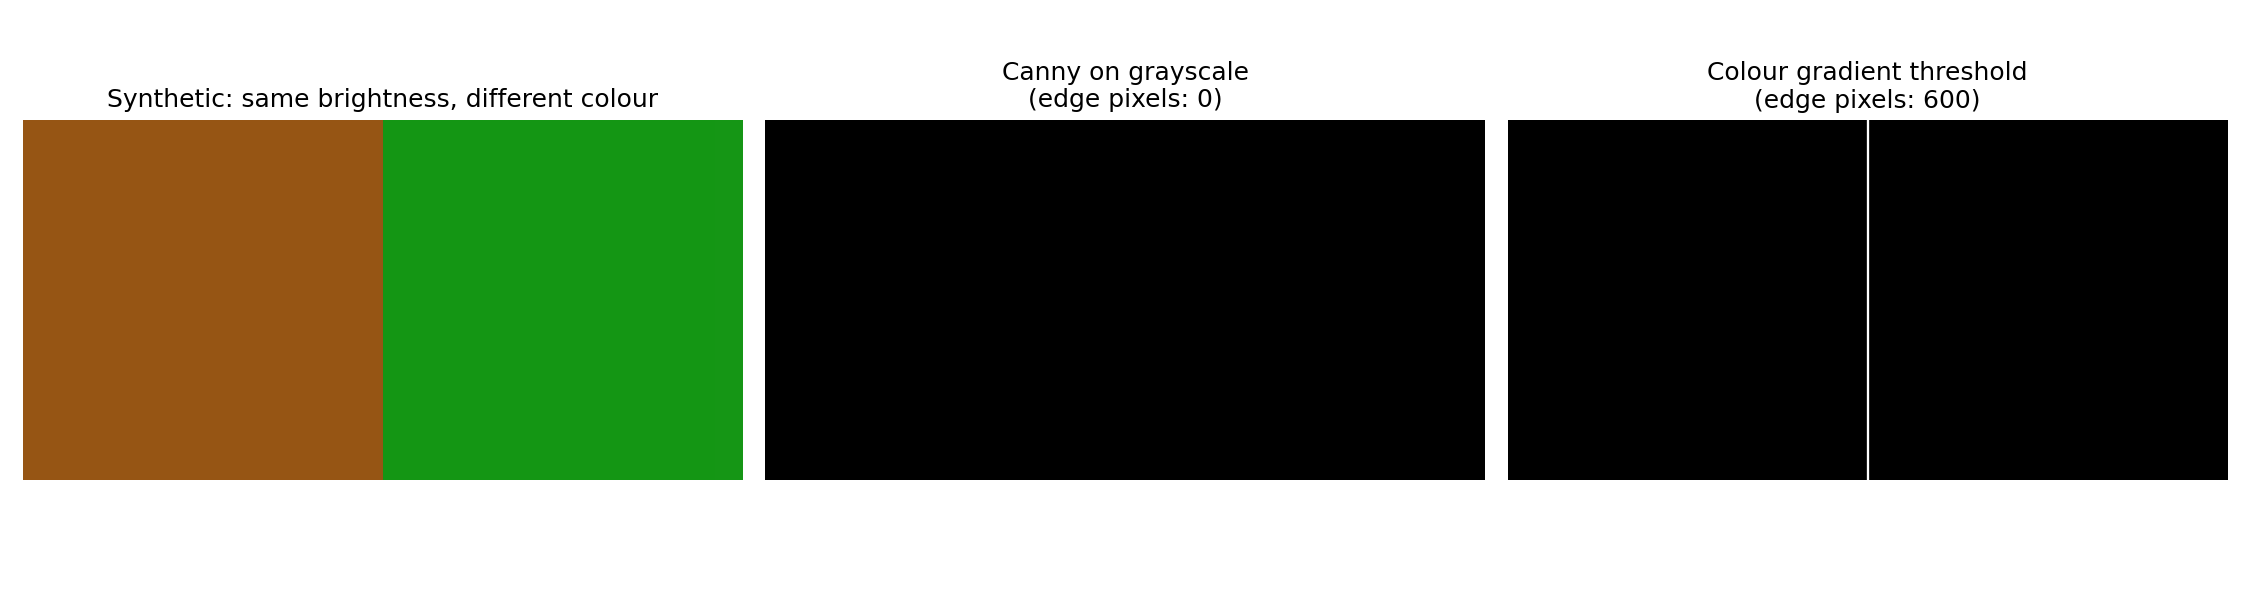
\includegraphics[width=0.75\linewidth]{outputs/synthetic_colour_vs_gray_edge.png}
    \caption{Synthetic image with identical brightness, different hue. Grayscale Canny finds no edge; color gradient threshold detects the boundary.}
    \label{fig:synthetic}
\end{figure}

\begin{figure}[H]
    \centering
    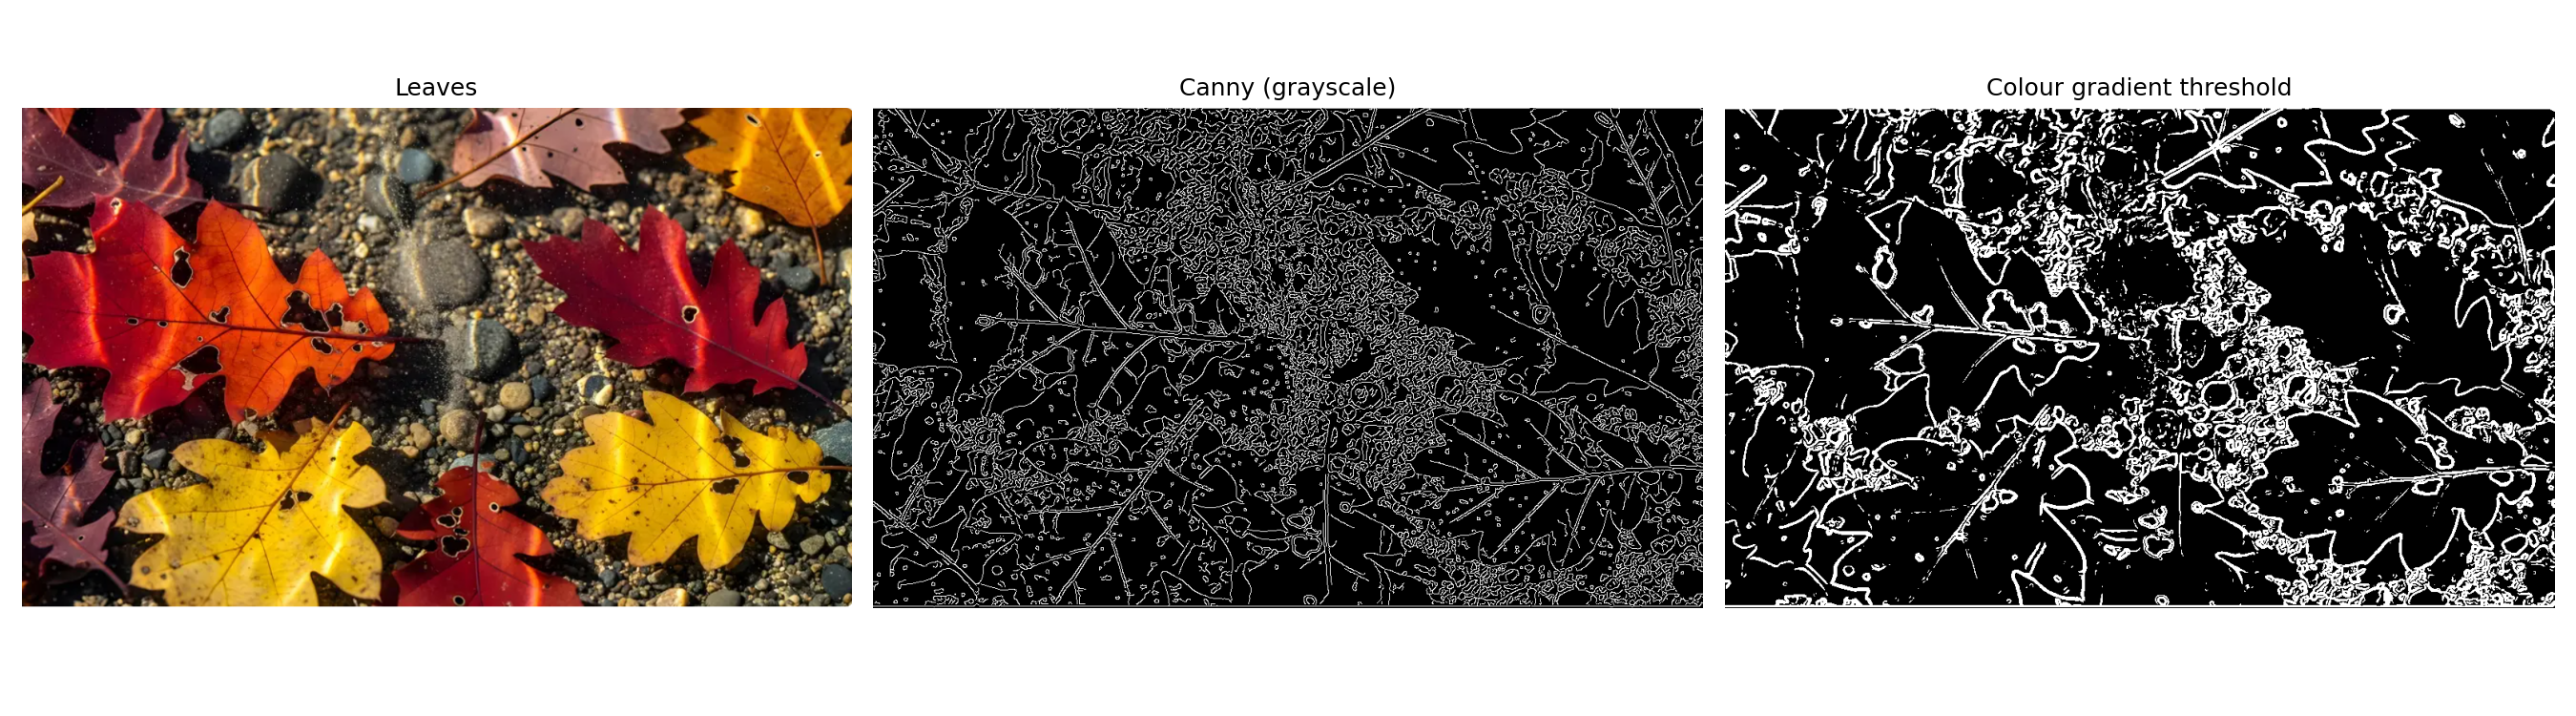
\includegraphics[width=0.97\linewidth]{outputs/leaves_colour_vs_gray_edge.png}
    \caption{Organic example (leaves): color gradient threshold reveals boundaries missed by grayscale Canny.}
    \label{fig:leaves_color_edge}
\end{figure}

\subsection{Discussion}

Figures~\ref{fig:synthetic} and~\ref{fig:leaves_color_edge} confirm that when two regions share the same luminance but differ in hue, standard grayscale processing produces \emph{no signal}.  The Di~Zenzo color gradient combines gradient information from all channels simultaneously; any color discontinuity --- even with zero luminance change --- produces a large $M$ value.

The active contour framework benefits directly: replacing $|\nabla I_{\mathrm{gray}}|$ with $M_{\mathrm{DiZenzo}}$ as the stopping function $g$ allows the contour to lock onto color boundaries that would be invisible in a grayscale-based snake.

% ============================================================
\section{Section 9 — Comprehensive Comparison}
% ============================================================

\subsection{Three methods on one image}

\begin{figure}[H]
    \centering
    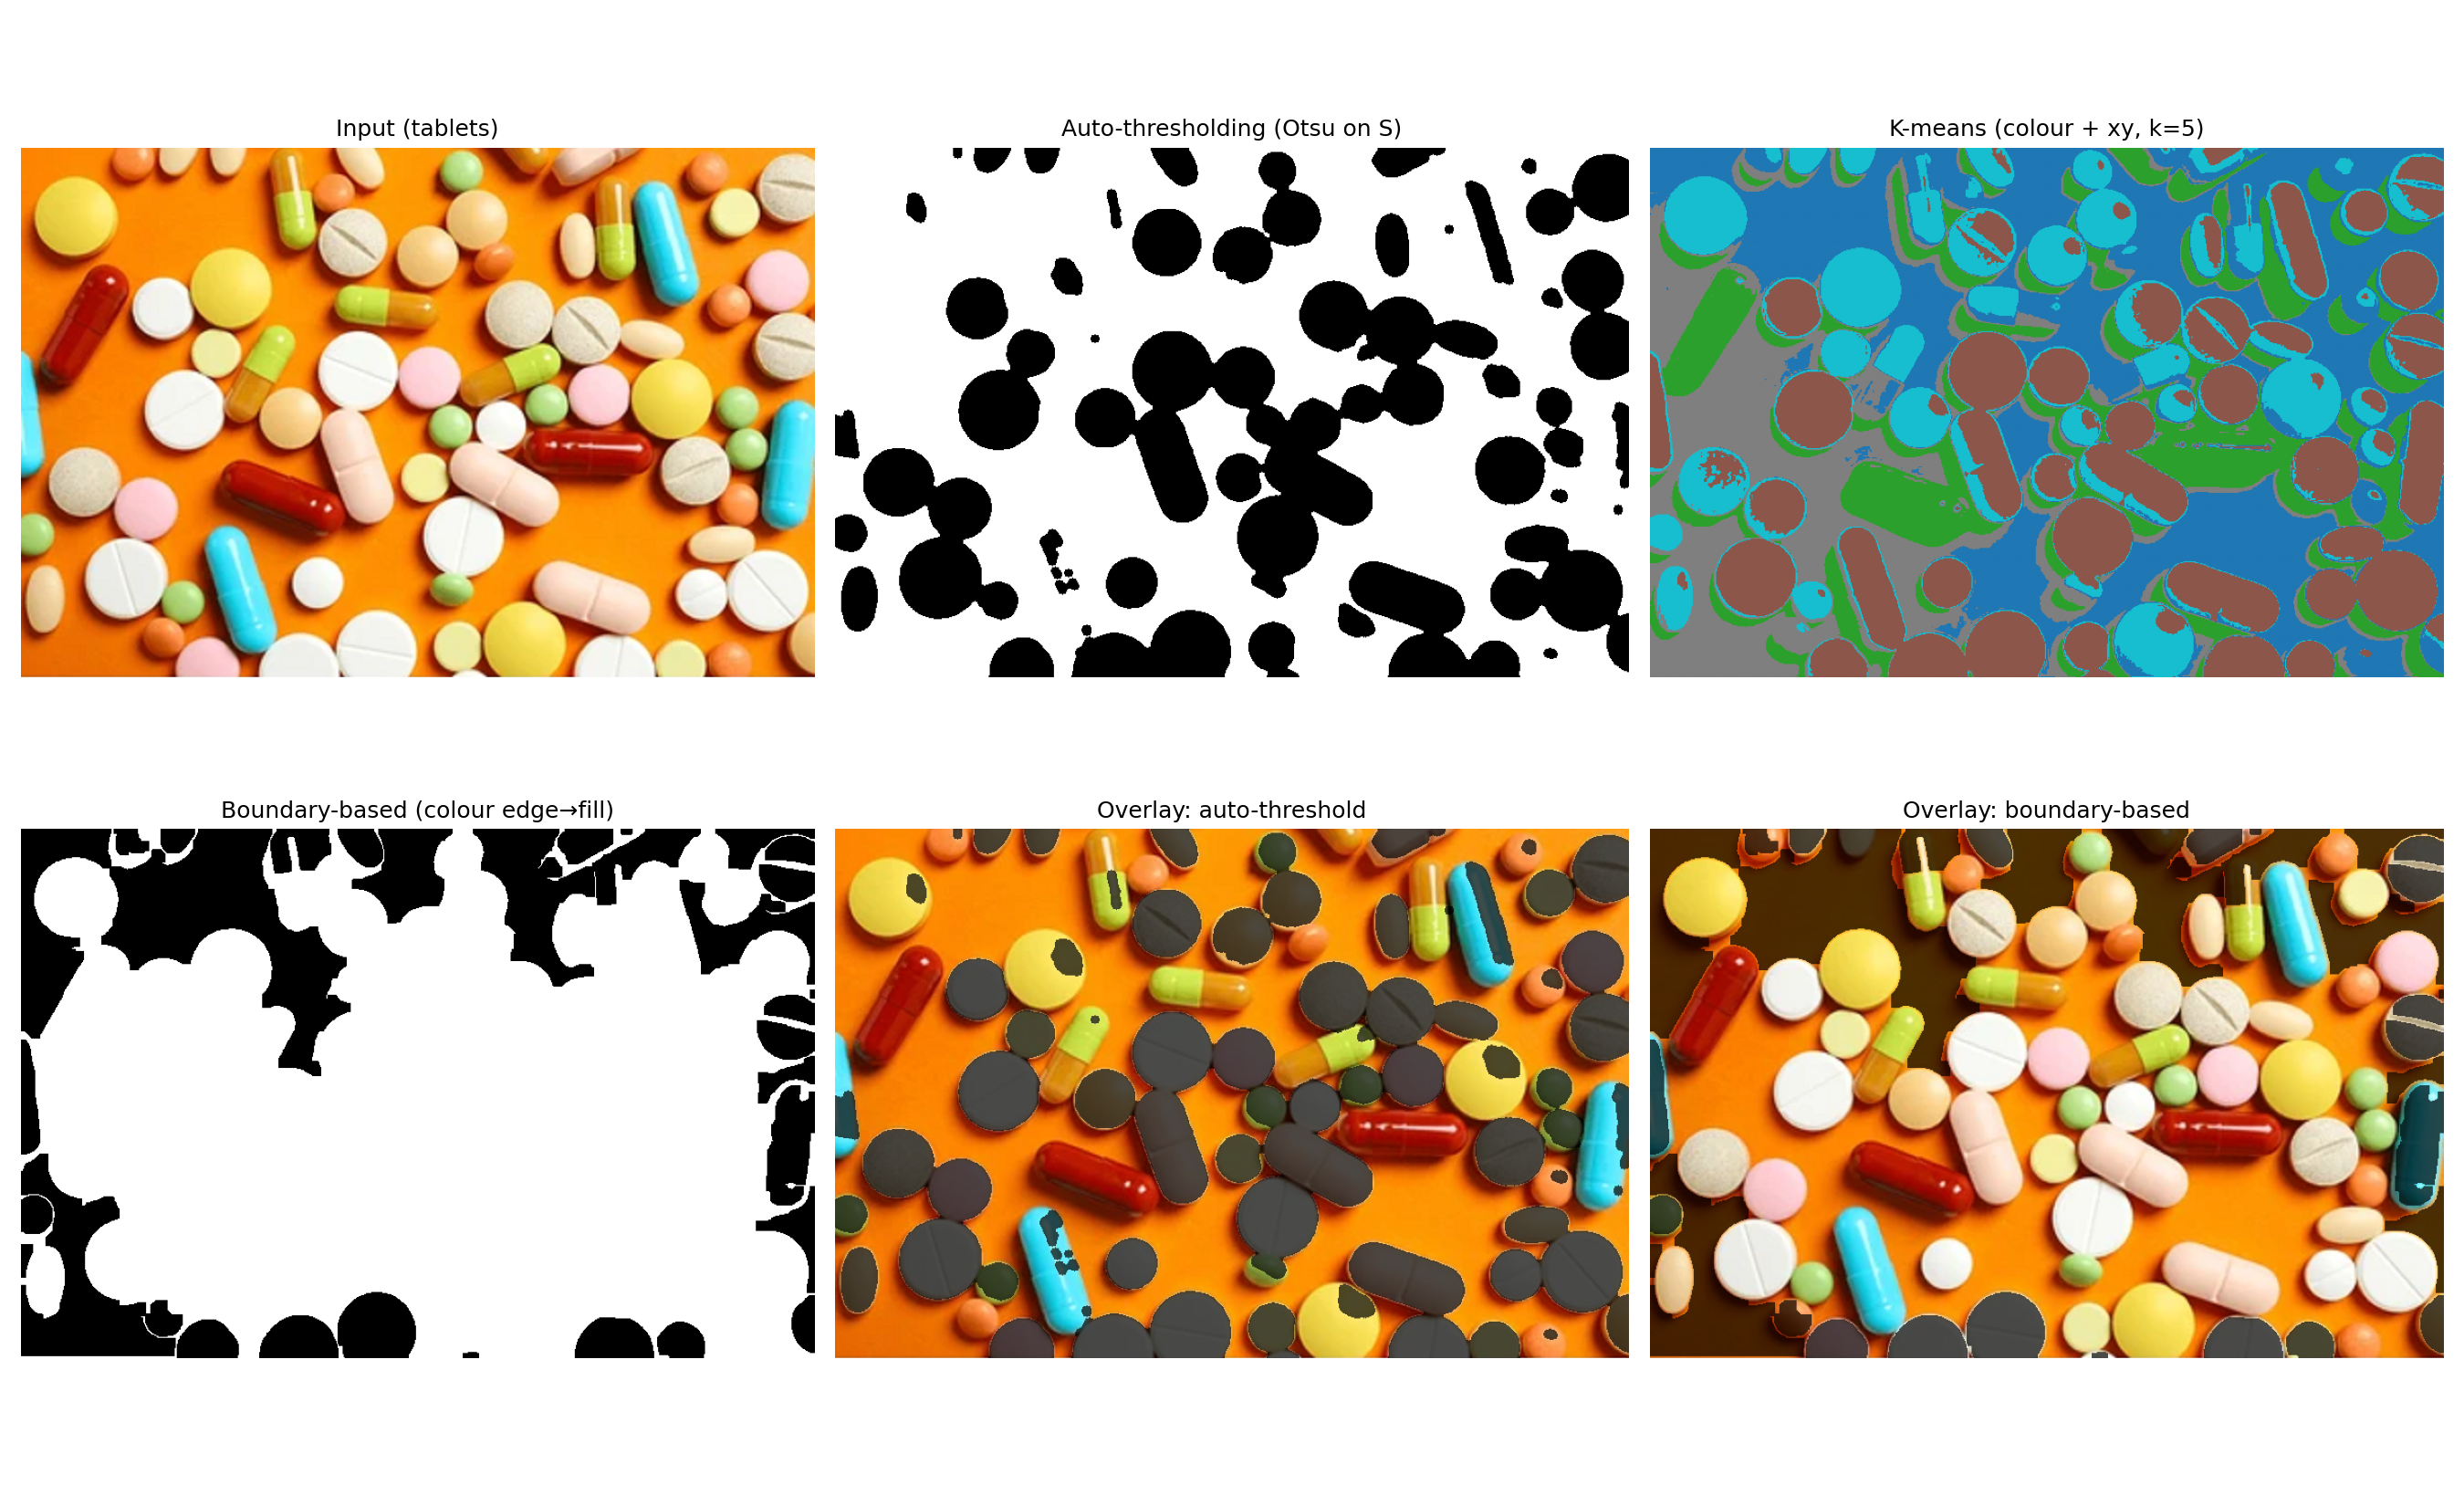
\includegraphics[width=0.97\linewidth]{outputs/comparison_three_methods.png}
    \caption{Auto-thresholding (Otsu on $S$), K-means with color+position, and boundary-based (color edge → fill) applied to \texttt{tablets4.png}.}
    \label{fig:three_methods}
\end{figure}

\begin{table}[H]
\centering
\caption{Qualitative comparison of the three paradigms.}
\label{tab:three_methods}
\begin{tabular}{p{3.2cm}p{4.8cm}p{4.8cm}}
\toprule
\textbf{Method} & \textbf{Strengths} & \textbf{Weaknesses} \\
\midrule
Auto-thresholding (Otsu on $S$) &
    Fast; no parameters except channel choice; excellent for colorful objects on gray background. &
    Single global threshold; fails with uneven illumination; cannot distinguish similarly-saturated objects. \\
\addlinespace
K-means (color+xy) &
    Handles multiple color classes; spatially coherent when $(x,y)$ is included; produces a full labeling. &
    Must choose $k$; nondeterministic; slow for large images; may split large objects. \\
\addlinespace
Boundary-based (edge→fill) &
    Preserves object shape faithfully; handles overlapping objects via contour extraction. &
    Sensitive to edge map quality; morphological close must be tuned; gaps in edges cause unfilled regions. \\
\bottomrule
\end{tabular}
\end{table}

\subsection{Equalization on $V$ vs.\ $L^*$ before thresholding}

\begin{figure}[H]
    \centering
    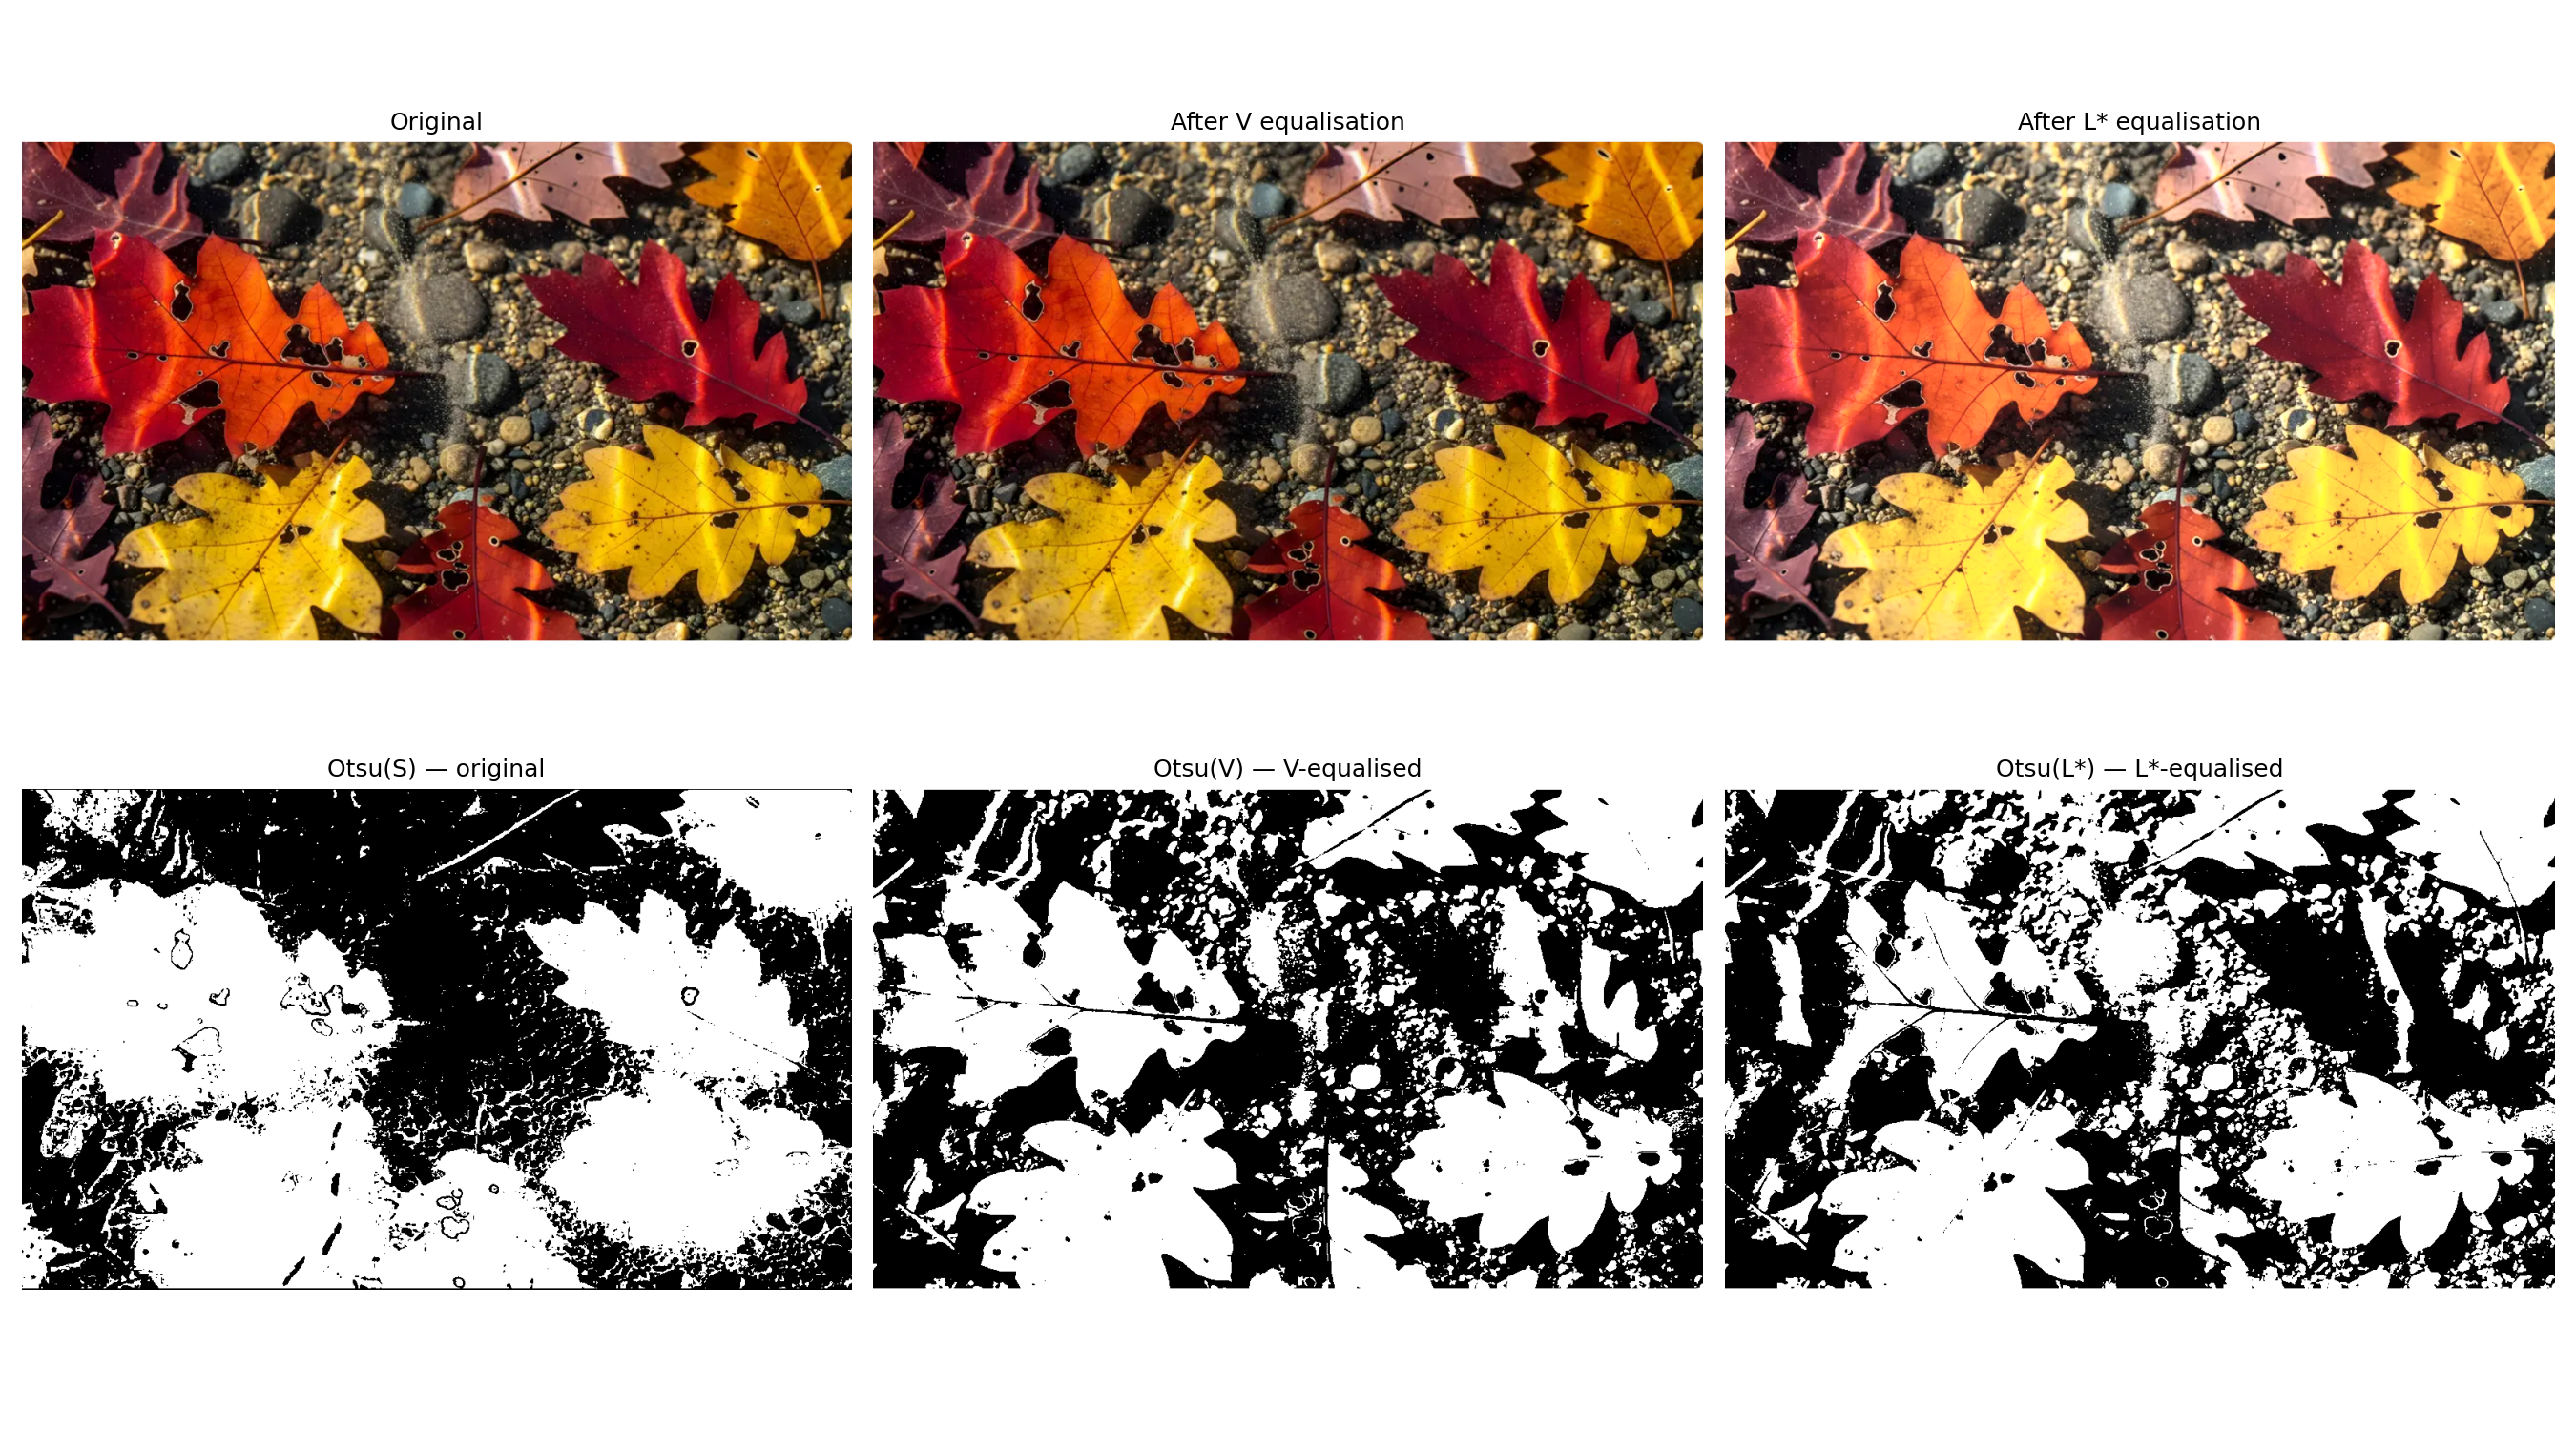
\includegraphics[width=0.97\linewidth]{outputs/equalization_V_vs_Lstar.png}
    \caption{Top: original, V-equalized, and $L^*$-equalized images. Bottom: Otsu masks after equalization on each channel.}
    \label{fig:equalise}
\end{figure}

Histogram equalization on $V$ redistributes brightness uniformly in HSV space, which can distort hue-saturation perception.  Equalizing $L^*$ in Lab space is more perceptually consistent because it modifies only the luminance axis while leaving chrominance ($a^*$, $b^*$) untouched.  For subsequent thresholding, $L^*$ equalization tends to produce cleaner separations when the foreground/background difference is primarily \emph{luminance-based}.

\subsection{When grayscale fails but color succeeds}

Three demonstrated cases:

\begin{enumerate}
    \item \textbf{Synthetic same-brightness two-region image} (Task 8.5.3): Both halves have $V=150$; grayscale Canny finds zero edges. Di~Zenzo color gradient detects the hue boundary.

    \item \textbf{Leaves image — intra-leaf boundaries} (Task 6.5.4): Adjacent leaves with similar luminance but different green hues. Grayscale Canny misses many inter-leaf edges; Lab-channel Canny captures them.

    \item \textbf{Tablets — color-only separation} (Task 5.7): Differentially colored tablets have overlapping grayscale distributions. Otsu on $S$ cleanly separates colorful tablets from the neutral background.
\end{enumerate}

The common theme: \emph{grayscale discards all chromatic information.}  Whenever the perceptual boundary between regions lies primarily in hue or saturation rather than luminance, any grayscale method will fail.

% ============================================================
\section{Conclusion}
% ============================================================

This lab explored the four main directions for color image analysis:

\begin{enumerate}
    \item \textbf{Auto-thresholding} --- Saturation $S$ is the most effective single channel for segmenting colorful objects; the two-step HSV pipeline and Lab color-distance thresholding further improve robustness.
    \item \textbf{Color edge detection} --- Di~Zenzo's vector-gradient framework and multi-channel Canny both capture edges invisible in grayscale.  The mini color Canny (NMS + hysteresis on the color magnitude) produces thinned, well-localized edges.
    \item \textbf{Region-based segmentation} --- Region growing in Lab is more stable than in RGB; K-means with spatial features produces compact, coherent regions.
    \item \textbf{Edge-based segmentation} --- Merging Canny on $L^*$ and $S$, closing gaps morphologically, and filling contours yields clean object masks.  Color gradient stopping functions are a natural improvement for active contour models.
\end{enumerate}

All implementations are contained in the companion notebook \texttt{lab08\_BuiQuangChien\_23001837.ipynb}.

\end{document}
